%%%%%%%%%%%%%%%%%%%%%%%%%%%%%%%%%%%%%%%%%%%%%%%%%%%%%%%%%%%%%%%
%% OXFORD THESIS TEMPLATE

% Use this template to produce a standard thesis that meets the Oxford University requirements for DPhil submission
%
% Originally by Keith A. Gillow (gillow@maths.ox.ac.uk), 1997
% Modified by Sam Evans (sam@samuelevansresearch.org), 2007
% Modified by John McManigle (john@oxfordechoes.com), 2015
% Modified by Ulrik Lyngs (ulrik.lyngs@cs.ox.ac.uk), 2018, for use with R Markdown
%
% Ulrik Lyngs, 25 Nov 2018: Following John McManigle, broad permissions are granted to use, modify, and distribute this software
% as specified in the MIT License included in this distribution's LICENSE file.
%
% John tried to comment this file extensively, so read through it to see how to use the various options.  Remember
% that in LaTeX, any line starting with a % is NOT executed.  Several places below, you have a choice of which line to use
% out of multiple options (eg draft vs final, for PDF vs for binding, etc.)  When you pick one, add a % to the beginning of
% the lines you don't want.


%%%%% CHOOSE PAGE LAYOUT
% The most common choices should be below.  You can also do other things, like replacing "a4paper" with "letterpaper", etc.

% This one will format for two-sided binding (ie left and right pages have mirror margins; blank pages inserted where needed):
%\documentclass[a4paper,twoside]{templates/ociamthesis}
% This one will format for one-sided binding (ie left margin > right margin; no extra blank pages):
%\documentclass[a4paper]{ociamthesis}
% This one will format for PDF output (ie equal margins, no extra blank pages):
%\documentclass[a4paper,nobind]{templates/ociamthesis}
%UL 2 Dec 2018: pass this in from YAML
\documentclass[a4paper, twoside]{templates/ociamthesis}


% UL 30 Nov 2018 pandoc puts lists in 'tightlist' command when no space between bullet points in Rmd file
\providecommand{\tightlist}{%
  \setlength{\itemsep}{0pt}\setlength{\parskip}{0pt}}
 
% UL 1 Dec 2018, fix to include code in shaded environments
\usepackage{color}
\usepackage{fancyvrb}
\newcommand{\VerbBar}{|}
\newcommand{\VERB}{\Verb[commandchars=\\\{\}]}
\DefineVerbatimEnvironment{Highlighting}{Verbatim}{commandchars=\\\{\}}
% Add ',fontsize=\small' for more characters per line
\usepackage{framed}
\definecolor{shadecolor}{RGB}{248,248,248}
\newenvironment{Shaded}{\begin{snugshade}}{\end{snugshade}}
\newcommand{\AlertTok}[1]{\textcolor[rgb]{0.94,0.16,0.16}{#1}}
\newcommand{\AnnotationTok}[1]{\textcolor[rgb]{0.56,0.35,0.01}{\textbf{\textit{#1}}}}
\newcommand{\AttributeTok}[1]{\textcolor[rgb]{0.77,0.63,0.00}{#1}}
\newcommand{\BaseNTok}[1]{\textcolor[rgb]{0.00,0.00,0.81}{#1}}
\newcommand{\BuiltInTok}[1]{#1}
\newcommand{\CharTok}[1]{\textcolor[rgb]{0.31,0.60,0.02}{#1}}
\newcommand{\CommentTok}[1]{\textcolor[rgb]{0.56,0.35,0.01}{\textit{#1}}}
\newcommand{\CommentVarTok}[1]{\textcolor[rgb]{0.56,0.35,0.01}{\textbf{\textit{#1}}}}
\newcommand{\ConstantTok}[1]{\textcolor[rgb]{0.00,0.00,0.00}{#1}}
\newcommand{\ControlFlowTok}[1]{\textcolor[rgb]{0.13,0.29,0.53}{\textbf{#1}}}
\newcommand{\DataTypeTok}[1]{\textcolor[rgb]{0.13,0.29,0.53}{#1}}
\newcommand{\DecValTok}[1]{\textcolor[rgb]{0.00,0.00,0.81}{#1}}
\newcommand{\DocumentationTok}[1]{\textcolor[rgb]{0.56,0.35,0.01}{\textbf{\textit{#1}}}}
\newcommand{\ErrorTok}[1]{\textcolor[rgb]{0.64,0.00,0.00}{\textbf{#1}}}
\newcommand{\ExtensionTok}[1]{#1}
\newcommand{\FloatTok}[1]{\textcolor[rgb]{0.00,0.00,0.81}{#1}}
\newcommand{\FunctionTok}[1]{\textcolor[rgb]{0.00,0.00,0.00}{#1}}
\newcommand{\ImportTok}[1]{#1}
\newcommand{\InformationTok}[1]{\textcolor[rgb]{0.56,0.35,0.01}{\textbf{\textit{#1}}}}
\newcommand{\KeywordTok}[1]{\textcolor[rgb]{0.13,0.29,0.53}{\textbf{#1}}}
\newcommand{\NormalTok}[1]{#1}
\newcommand{\OperatorTok}[1]{\textcolor[rgb]{0.81,0.36,0.00}{\textbf{#1}}}
\newcommand{\OtherTok}[1]{\textcolor[rgb]{0.56,0.35,0.01}{#1}}
\newcommand{\PreprocessorTok}[1]{\textcolor[rgb]{0.56,0.35,0.01}{\textit{#1}}}
\newcommand{\RegionMarkerTok}[1]{#1}
\newcommand{\SpecialCharTok}[1]{\textcolor[rgb]{0.00,0.00,0.00}{#1}}
\newcommand{\SpecialStringTok}[1]{\textcolor[rgb]{0.31,0.60,0.02}{#1}}
\newcommand{\StringTok}[1]{\textcolor[rgb]{0.31,0.60,0.02}{#1}}
\newcommand{\VariableTok}[1]{\textcolor[rgb]{0.00,0.00,0.00}{#1}}
\newcommand{\VerbatimStringTok}[1]{\textcolor[rgb]{0.31,0.60,0.02}{#1}}
\newcommand{\WarningTok}[1]{\textcolor[rgb]{0.56,0.35,0.01}{\textbf{\textit{#1}}}}
%UL 2 Dec 2018 add a bit of white space before and after code blocks
\renewenvironment{Shaded}
{
  \vspace{4pt}%
  \begin{snugshade}%
}{%
  \end{snugshade}%
  \vspace{4pt}%
}

%UL 2 Dec 2018 reduce whitespace around verbatim environments
\usepackage{etoolbox}
\makeatletter
\preto{\@verbatim}{\topsep=0pt \partopsep=0pt }
\makeatother

%UL 26 Mar 2019, enable strikethrough
\usepackage[normalem]{ulem}

%UL 15 Oct 2019, enable link highlighting to be turned off from YAML
\usepackage[colorlinks=false,pdfpagelabels,hidelinks=true]{hyperref}

%%%%% SELECT YOUR DRAFT OPTIONS
% Three options going on here; use in any combination.  But remember to turn the first two off before
% generating a PDF to send to the printer!

% This adds a "DRAFT" footer to every normal page.  (The first page of each chapter is not a "normal" page.)
\fancyfoot[C]{\emph{DRAFT Printed on \today}}

% This highlights (in blue) corrections marked with (for words) \mccorrect{blah} or (for whole
% paragraphs) \begin{mccorrection} . . . \end{mccorrection}.  This can be useful for sending a PDF of
% your corrected thesis to your examiners for review.  Turn it off, and the blue disappears.
\correctionstrue

%%%%% BIBLIOGRAPHY SETUP
% Note that your bibliography will require some tweaking depending on your department, preferred format, etc.
% The options included below are just very basic "sciencey" and "humanitiesey" options to get started.
% If you've not used LaTeX before, I recommend reading a little about biblatex/biber and getting started with it.
% If you're already a LaTeX pro and are used to natbib or something, modify as necessary.
% Either way, you'll have to choose and configure an appropriate bibliography format...

% The science-type option: numerical in-text citation with references in order of appearance.
% \usepackage[style=numeric-comp, sorting=none, backend=biber, doi=false, isbn=false]{biblatex}
% \newcommand*{\bibtitle}{References}

% The humanities-type option: author-year in-text citation with an alphabetical works cited.
% \usepackage[style=authoryear, sorting=nyt, backend=biber, maxcitenames=2, useprefix, doi=false, isbn=false]{biblatex}
% \newcommand*{\bibtitle}{Works Cited}

%UL 3 Dec 2018: set this from YAML in index.Rmd
\usepackage[style=apa, sorting=nyt, backend=biber, maxcitenames=2, useprefix, doi=true, isbn=false, uniquename=false]{biblatex}
\newcommand*{\bibtitle}{Works Cited}


% This makes the bibliography left-aligned (not 'justified') and slightly smaller font.
\renewcommand*{\bibfont}{\raggedright\small}

% Change this to the name of your .bib file (usually exported from a citation manager like Zotero or EndNote).
\addbibresource{references.bib}


% Uncomment this if you want equation numbers per section (2.3.12), instead of per chapter (2.18):
%\numberwithin{equation}{subsection}


%%%%% THESIS / TITLE PAGE INFORMATION
% Everybody needs to complete the following:
\title{My thesis title\\
Title second row}
\author{Shiran Koifman}
\college{}

% Master's candidates who require the alternate title page (with candidate number and word count)
% must also un-comment and complete the following three lines:
%\masterssubmissiontrue
%\candidateno{933516}
%\wordcount{28,815}

% Uncomment the following line if your degree also includes exams (eg most masters):
%\renewcommand{\submittedtext}{Submitted in partial completion of the}
% Your full degree name.  (But remember that DPhils aren't "in" anything.  They're just DPhils.)
\degree{}
% Term and year of submission, or date if your board requires (eg most masters)
\degreedate{January 15 2021}


%%%%% YOUR OWN PERSONAL MACROS
% This is a good place to dump your own LaTeX macros as they come up.

% To make text superscripts shortcuts
	\renewcommand{\th}{\textsuperscript{th}} % ex: I won 4\th place
	\newcommand{\nd}{\textsuperscript{nd}}
	\renewcommand{\st}{\textsuperscript{st}}
	\newcommand{\rd}{\textsuperscript{rd}}

%%%%% THE ACTUAL DOCUMENT STARTS HERE
\begin{document}

%%%%% CHOOSE YOUR LINE SPACING HERE
% This is the official option.  Use it for your submission copy and library copy:
\setlength{\textbaselineskip}{22pt plus2pt}
% This is closer spacing (about 1.5-spaced) that you might prefer for your personal copies:
%\setlength{\textbaselineskip}{18pt plus2pt minus1pt}

% You can set the spacing here for the roman-numbered pages (acknowledgements, table of contents, etc.)
\setlength{\frontmatterbaselineskip}{17pt plus1pt minus1pt}

% UL: You can set the line and paragraph spacing here for the separate abstract page to be handed in to Examination schools
\setlength{\abstractseparatelineskip}{13pt plus1pt minus1pt}
\setlength{\abstractseparateparskip}{0pt plus 1pt}

% UL: You can set the general paragraph spacing here - I've set it to 2pt (was 0) so
% it's less claustrophobic
\setlength{\parskip}{2pt plus 1pt}


% Leave this line alone; it gets things started for the real document.
\setlength{\baselineskip}{\textbaselineskip}


%%%%% CHOOSE YOUR SECTION NUMBERING DEPTH HERE
% You have two choices.  First, how far down are sections numbered?  (Below that, they're named but
% don't get numbers.)  Second, what level of section appears in the table of contents?  These don't have
% to match: you can have numbered sections that don't show up in the ToC, or unnumbered sections that
% do.  Throughout, 0 = chapter; 1 = section; 2 = subsection; 3 = subsubsection, 4 = paragraph...

% The level that gets a number:
\setcounter{secnumdepth}{2}
% The level that shows up in the ToC:
\setcounter{tocdepth}{2}


%%%%% ABSTRACT SEPARATE
% This is used to create the separate, one-page abstract that you are required to hand into the Exam
% Schools.  You can comment it out to generate a PDF for printing or whatnot.

% JEM: Pages are roman numbered from here, though page numbers are invisible until ToC.  This is in
% keeping with most typesetting conventions.
\begin{romanpages}

% Title page is created here
\maketitle

%%%%% DEDICATION -- If you'd like one, un-comment the following.
\begin{dedication}
  For Yihui Xie
\end{dedication}

%%%%% ACKNOWLEDGEMENTS -- Nothing to do here except comment out if you don't want it.
\begin{acknowledgements}
 	This is where you will normally thank your advisor, colleagues, family and friends, as well as funding and institutional support. In our case, we will give our praises to the people who developed the ideas and tools that allow us to push open science a little step forward by writing plain-text, transparent, and reproducible theses in R Markdown.

  We must be grateful to John Gruber for inventing the original version of Markdown, to John MacFarlane for creating Pandoc (\url{http://pandoc.org}) which converts Markdown to a large number of output formats, and to Yihui Xie for creating \texttt{knitr} which introduced R Markdown as a way of embedding code in Markdown documents, and \texttt{bookdown} which added tools for technical and longer-form writing.

  Special thanks to \href{http://chester.rbind.io}{Chester Ismay}, who created the \texttt{thesisdown} package that helped many a PhD student write their theses in R Markdown. And a very special tahnks to John McManigle, whose adaption of Sam Evans' adaptation of Keith Gillow's original maths template for writing an Oxford University DPhil thesis in \LaTeX~provided the template that I adapted for R Markdown.

  Finally, profuse thanks to JJ Allaire, the founder and CEO of \href{http://rstudio.com}{RStudio}, and Hadley Wickham, the mastermind of the tidyverse without whom we'd all just given up and done data science in Python instead. Thanks for making data science easier, more accessible, and more fun for us all.

  \begin{flushright}
  Ulrik Lyngs \\
  Linacre College, Oxford \\
  2 December 2018
  \end{flushright}
\end{acknowledgements}


%%%%% ABSTRACT -- Nothing to do here except comment out if you don't want it.
\begin{abstract}
	This \emph{R Markdown} template is for writing an Oxford University thesis. The template is built using Yihui Xie's \texttt{bookdown} package, with heavy inspiration from Chester Ismay's \texttt{thesisdown} and the \texttt{OxThesis} \LaTeX~template (most recently adapted by John McManigle).

 This template's sample content include illustrations of how to write a thesis in R Markdown, and largely follows the structure from \href{https://ulyngs.github.io/rmarkdown-workshop-2019/}{this R Markdown workshop}.

 Congratulations for taking a step further into the lands of open, reproducible science by writing your thesis using a tool that allows you to transparently include tables and dynamically generated plots directly from the underlying data. Hip hooray!
\end{abstract}

%%%%% MINI TABLES
% This lays the groundwork for per-chapter, mini tables of contents.  Comment the following line
% (and remove \minitoc from the chapter files) if you don't want this.  Un-comment either of the
% next two lines if you want a per-chapter list of figures or tables.
  \dominitoc % include a mini table of contents

% This aligns the bottom of the text of each page.  It generally makes things look better.
\flushbottom

% This is where the whole-document ToC appears:
\tableofcontents

\listoffigures
	\mtcaddchapter
  	% \mtcaddchapter is needed when adding a non-chapter (but chapter-like) entity to avoid confusing minitoc

% Uncomment to generate a list of tables:
\listoftables
  \mtcaddchapter
%%%%% LIST OF ABBREVIATIONS
% This example includes a list of abbreviations.  Look at text/abbreviations.tex to see how that file is
% formatted.  The template can handle any kind of list though, so this might be a good place for a
% glossary, etc.
% First parameter can be changed eg to "Glossary" or something.
% Second parameter is the max length of bold terms.
\begin{mclistof}{List of Abbreviations}{3.2cm}

\item[1-D, 2-D] One- or two-dimensional, referring in this thesis to spatial dimensions in an image.

\item[Otter] One of the finest of water mammals.

\item[Hedgehog] Quite a nice prickly friend.

\end{mclistof} 


% The Roman pages, like the Roman Empire, must come to its inevitable close.
\end{romanpages}

%%%%% CHAPTERS
% Add or remove any chapters you'd like here, by file name (excluding '.tex'):
\flushbottom

% all your chapters and appendices will appear here
\hypertarget{introduction}{%
\chapter*{Introduction}\label{introduction}}
\addcontentsline{toc}{chapter}{Introduction}

\adjustmtc

Welcome to the \emph{R Markdown} Oxford University thesis template.
This sample content is adapted from \href{https://github.com/ismayc/thesisdown}{\texttt{thesisdown}} and the formatting of PDF output is adapted from the \href{https://github.com/mcmanigle/OxThesis}{OxThesis LaTeX template}.
Hopefully, writing your thesis in R Markdown will provide a nicer interface to the OxThesis template if you haven't used TeX or LaTeX before.
More importantly, using \emph{R Markdown} allows you to embed chunks of code directly into your thesis and generate plots and tables directly from the underlying data, avoiding copy-paste steps.
This will get you into the habit of doing reproducible research, which benefits you long-term as a researcher, but also will greatly help anyone that is trying to reproduce or build upon your results down the road.

Using LaTeX together with \emph{Markdown} is more consistent than the output of a word processor, much less prone to corruption or crashing, and the resulting file is smaller than a Word file.
While you may never have had problems using Word in the past, your thesis is likely going to be about twice as large and complex as anything you've written before, taxing Word's capabilities.

\hypertarget{speech-in-noise-in-children}{%
\section*{Speech-in-noise in children}\label{speech-in-noise-in-children}}
\addcontentsline{toc}{section}{Speech-in-noise in children}

\emph{R Markdown} creates a simple and straightforward way to interface with the beauty of LaTeX.
Packages have been written in \textbf{R} to work directly with LaTeX to produce nicely formatting tables and paragraphs.
In addition to creating a user friendly interface to LaTeX, \emph{R Markdown} allows you to read in your data, analyze it and to visualize it using \textbf{R}, \textbf{Python} or other languages, and provide documentation and commentary on the results of your project.\\
Further, it allows for results of code output to be passed inline to the commentary of your results.
You'll see more on this later, focusing on \textbf{R}. If you are more into \textbf{Python} or something else, you can still use \emph{R Markdown} - see \href{https://bookdown.org/yihui/rmarkdown/language-engines.html}{`Other language engines'} in Yihui Xie's \href{https://bookdown.org/yihui/rmarkdown/language-engines.html}{\emph{R Markdown: The Definitive Guide}}.

\hypertarget{apd-definition}{%
\section*{APD definition}\label{apd-definition}}
\addcontentsline{toc}{section}{APD definition}

Anyone who needs to use data analysis, math, tables, a lot of figures, complex cross-references, or who just cares about reproducibility in research can benefit from using \emph{R Markdown}.
If you are working in `softer' fields, the user-friendly nature of the \emph{Markdown} syntax and its ability to keep track of and easily include figures, automatically generate a table of contents, index, references, table of figures, etc. should still make it of great benefit to your thesis project.

\hypertarget{diagnosis}{%
\section*{Diagnosis}\label{diagnosis}}
\addcontentsline{toc}{section}{Diagnosis}

Anyone who needs to use data analysis, math, tables, a lot of figures, complex cross-references, or who just cares about reproducibility in research can benefit from using \emph{R Markdown}.
If you are working in `softer' fields, the user-friendly nature of the \emph{Markdown} syntax and its ability to keep track of and easily include figures, automatically generate a table of contents, index, references, table of figures, etc. should still make it of great benefit to your thesis project.

\hypertarget{binaural-and-spatial-listening-in-apd}{%
\section*{Binaural and spatial listening in APD}\label{binaural-and-spatial-listening-in-apd}}
\addcontentsline{toc}{section}{Binaural and spatial listening in APD}

Anyone who needs to use data analysis, math, tables, a lot of figures, complex cross-references, or who just cares about reproducibility in research can benefit from using \emph{R Markdown}.
If you are working in `softer' fields, the user-friendly nature of the \emph{Markdown} syntax and its ability to keep track of and easily include figures, automatically generate a table of contents, index, references, table of figures, etc. should still make it of great benefit to your thesis project.

\hypertarget{summary}{%
\section*{Summary}\label{summary}}
\addcontentsline{toc}{section}{Summary}

Anyone who needs to use data analysis, math, tables, a lot of figures, complex cross-references, or who just cares about reproducibility in research can benefit from using \emph{R Markdown}.
If you are working in `softer' fields, the user-friendly nature of the \emph{Markdown} syntax and its ability to keep track of and easily include figures, automatically generate a table of contents, index, references, table of figures, etc. should still make it of great benefit to your thesis project.

\begin{savequote}
Neque porro quisquam est qui dolorem ipsum quia dolor sit amet,
consectetur, adipisci velit\ldots{}

There is no one who loves pain itself, who seeks after it and wants to
have it, simply because it is pain\ldots{}
\qauthor{--- Cicero's \emph{de Finibus Bonorum et Malorum}.}\end{savequote}



\hypertarget{rmd-basics}{%
\chapter{Binaural listening: interripted and alternated speech-in-noise in adults}\label{rmd-basics}}

\minitoc 

Here is a brief introduction to using \emph{R Markdown}.
\emph{Markdown} is a simple formatting syntax for authoring HTML, PDF, and MS Word documents and much, much more.
\emph{R Markdown} provides the flexibility of \emph{Markdown} with the implementation of \textbf{R} input and output. For more details on using \emph{R Markdown} see \url{http://rmarkdown.rstudio.com}.

Be careful with your spacing in \emph{Markdown} documents.
While whitespace largely is ignored, it does at times give \emph{Markdown} signals as to how to proceed.
As a habit, try to keep everything left aligned whenever possible, especially as you type a new paragraph.
In other words, there is no need to indent basic text in the Rmd document (in fact, it might cause your text to do funny things if you do).

\hypertarget{influence-of-distractor-type-on-im}{%
\section{Influence of distractor type on IM}\label{influence-of-distractor-type-on-im}}

\hypertarget{introduction-1}{%
\subsection{Introduction}\label{introduction-1}}

\begin{itemize}
\tightlist
\item
  \emph{Italics} are done like *this* or \_this\_
\item
  \textbf{Bold} is done like **this** or \_\_this\_\_
\item
  \textbf{\emph{Bold and italics}} is done like ***this***, \_\_\_this\_\_\_, or (the most transparent solution, in my opinion) **\_this\_**
\end{itemize}

\hypertarget{experiment-i-speech-vs.-non-speech-distractors}{%
\subsection{Experiment I: speech vs.~non-speech distractors}\label{experiment-i-speech-vs.-non-speech-distractors}}

\begin{itemize}
\tightlist
\item
  \texttt{Inline\ code} is created with backticks like \texttt{\textasciigrave{}this\textasciigrave{}}
\end{itemize}

\hypertarget{methods}{%
\subsubsection{Methods}\label{methods}}

Sub\textsubscript{2} and super\textsuperscript{2} script is created like this\textasciitilde2\textasciitilde{} and this\^{}2\^{}

\hypertarget{results}{%
\subsubsection{Results}\label{results}}

\begin{itemize}
\tightlist
\item
  \sout{Strikethrough} is done \textasciitilde\textasciitilde like this\textasciitilde\textasciitilde{}
\end{itemize}

\hypertarget{discussion}{%
\subsubsection{Discussion}\label{discussion}}

\begin{itemize}
\tightlist
\item
  To include an actual *, \_ or \textbackslash, add another \textbackslash{} in front of them: \textbackslash*, \textbackslash\_, \textbackslash\textbackslash{}
\end{itemize}

\hypertarget{experiment-ii-speech-distractors-spoken-in-a-familiar-vs.-unfamiliar-language}{%
\subsection{Experiment II: speech distractors spoken in a familiar vs.~unfamiliar language}\label{experiment-ii-speech-distractors-spoken-in-a-familiar-vs.-unfamiliar-language}}

\begin{itemize}
\tightlist
\item
  -- and --- with -\/- and -\/-\/-
\end{itemize}

\hypertarget{methods-1}{%
\subsubsection{Methods}\label{methods-1}}

Do like this:

\begin{quote}
Put a \textgreater{} in front of the line.
\end{quote}

\hypertarget{results-1}{%
\subsubsection{Results}\label{results-1}}

\begin{itemize}
\tightlist
\item
  are done with \#'s of increasing number, i.e.~

  \begin{itemize}
  \tightlist
  \item
    \# First-level heading
  \item
    \#\# Second-level heading
  \item
    \#\#\# Etc.
  \end{itemize}
\end{itemize}

In PDF output, a level-five heading will turn into a paragraph heading, i.e.~\texttt{\textbackslash{}paragraph\{My\ level-five\ heading\}}, which appears as bold text on the same line as the subsequent paragraph.

\hypertarget{discussion-1}{%
\subsubsection{Discussion}\label{discussion-1}}

Unordered list by starting a line with an * or a -:

\begin{itemize}
\tightlist
\item
  Item 1
\item
  Item 2
\end{itemize}

Ordered lists by starting a line with a number:

\begin{enumerate}
\def\labelenumi{\arabic{enumi}.}
\tightlist
\item
  Item 1
\item
  Item 2
\end{enumerate}

Notice that you can mislabel the numbers and \emph{Markdown} will still make the order right in the output.

To create a sublist, indent the values a bit (at least four spaces or a tab):

\begin{enumerate}
\def\labelenumi{\arabic{enumi}.}
\tightlist
\item
  Item 1
\item
  Item 2
\item
  Item 3

  \begin{itemize}
  \tightlist
  \item
    Item 3a
  \item
    Item 3b
  \end{itemize}
\end{enumerate}

\hypertarget{general-discussion-and-conclusion}{%
\subsection{General discussion and conclusion}\label{general-discussion-and-conclusion}}

The official \emph{Markdown} way to create line breaks is by ending a line with more than two spaces.

Roses are red.
Violets are blue.

This appears on the same line in the output, because we didn't add spaces after red.

Roses are red.\\
Violets are blue.

This appears with a line break because I added spaces after red.

I find this is confusing, so I recommend the alternative way: Ending a line with a backslash will also create a linebreak:

Roses are red.\\
Violets are blue.

To create a new paragraph, you put a blank line.

Therefore, this line starts its own paragraph.

\hypertarget{dichotic-vs.-monotic-presentation-and-the-influence-of-speech-material}{%
\section{Dichotic vs.~monotic presentation and the influence of speech material}\label{dichotic-vs.-monotic-presentation-and-the-influence-of-speech-material}}

\begin{itemize}
\tightlist
\item
  \href{https://www.google.com}{This is a hyperlink} created by writing the text you want turned into a clickable link in \texttt{{[}square\ brackets\ followed\ by\ a{]}(https://hyperlink-in-parentheses)}
\end{itemize}

\hypertarget{introduction-2}{%
\subsection{Introduction}\label{introduction-2}}

\begin{itemize}
\tightlist
\item
  Are created\footnote{my footnote text} by writing either \^{}{[}my footnote text{]} for supplying the footnote content inline, or something like \texttt{{[}\^{}a-random-footnote-label{]}} and supplying the text elsewhere in the format shown below \footnote{This is a random test.}:
\end{itemize}

\texttt{{[}\^{}a-random-footnote-label{]}:\ This\ is\ a\ random\ test.}

\hypertarget{methods-2}{%
\subsection{Methods}\label{methods-2}}

To write comments within your text that won't actually be included in the output, use the same syntax as for writing comments in HTML. That is, \textless!-\/- this will not be included in the output -\/-\textgreater.

\hypertarget{results-2}{%
\subsection{Results}\label{results-2}}

The syntax for writing math is stolen from LaTeX. To write a math expression that will be shown \textbf{inline}, enclose it in dollar signs.
- This: \$A = \textbackslash pi*r\^{}\{2\}\$ Becomes: \(A = \pi*r^{2}\)

To write a math expression that will be shown in a block, enclose it in two dollar signs.\\
This: \$\$A = \textbackslash pi*r\^{}\{2\}\$\$

Becomes:
\[A = \pi*r^{2}\]

To create numbered equations, put them in an `equation' environment and give them a label with the syntax \texttt{(\textbackslash{}\#eq:label)}, like this:

\begin{Shaded}
\begin{Highlighting}[]
\KeywordTok{\textbackslash{}begin}\NormalTok{\{}\ExtensionTok{equation}\NormalTok{\}}\SpecialStringTok{ }
\SpecialStringTok{  f}\SpecialCharTok{\textbackslash{}left}\SpecialStringTok{(k}\SpecialCharTok{\textbackslash{}right}\SpecialStringTok{) = }\SpecialCharTok{\textbackslash{}binom}\SpecialStringTok{\{n\}\{k\} p\^{}k}\SpecialCharTok{\textbackslash{}left}\SpecialStringTok{(1{-}p}\SpecialCharTok{\textbackslash{}right}\SpecialStringTok{)\^{}\{n{-}k\}}
\SpecialStringTok{  (}\SpecialCharTok{\textbackslash{}\#}\SpecialStringTok{eq:binom)}
\KeywordTok{\textbackslash{}end}\NormalTok{\{}\ExtensionTok{equation}\NormalTok{\} }
\end{Highlighting}
\end{Shaded}

Becomes:
\begin{equation}
f\left(k\right)=\binom{n}{k}p^k\left(1-p\right)^{n-k}
\label{eq:binom}
\end{equation}

For more (e.g.~how to theorems), see e.g.~the documentation on \href{https://bookdown.org/yihui/bookdown/markdown-extensions-by-bookdown.html\#equations}{bookdown.org}

\hypertarget{discussion-2}{%
\subsection{Discussion}\label{discussion-2}}

\begin{itemize}
\item
  \emph{R Markdown: The Definitive Guide} - \url{https://bookdown.org/yihui/rmarkdown/}
\item
  \emph{R for Data Science} - \url{https://r4ds.had.co.nz}
\end{itemize}

\hypertarget{conclusion}{%
\subsection{Conclusion}\label{conclusion}}

\hypertarget{Chpt2}{%
\chapter{Spatial listening: development and normalisation of a children's spatialised speech-in-noise test}\label{Chpt2}}

\minitoc 

The magic of R Markdown is that we can add code within our document to make it dynamic.

We do this either as \emph{code chunks} (generally used for loading libraries and data, performing calculations, and adding images, plots, and tables), or \emph{inline code} (generally used for dynamically reporting results within our text).

\hypertarget{introduction-3}{%
\section{Introduction}\label{introduction-3}}

\hypertarget{methods-3}{%
\section{Methods}\label{methods-3}}

\hypertarget{discussion-3}{%
\section{Discussion}\label{discussion-3}}

\hypertarget{conclusion-1}{%
\section{Conclusion}\label{conclusion-1}}

The syntax of a code chunk is shown in Figure \ref{fig:chunk-parts}.

\begin{figure}
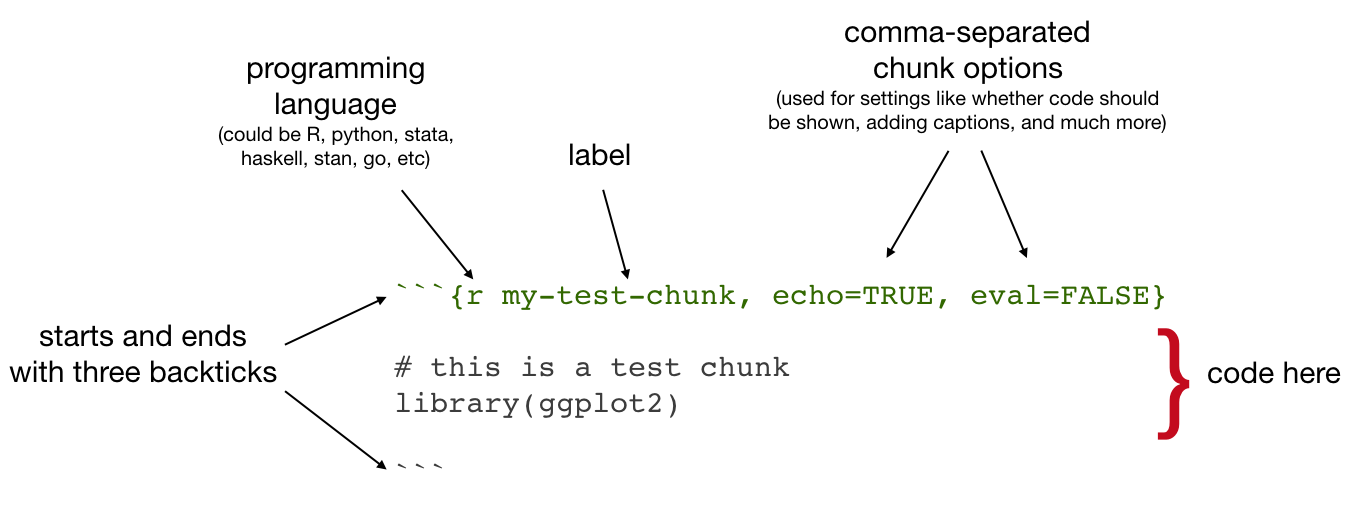
\includegraphics[width=1\linewidth]{figures/chunk-parts} \caption{Code chunk syntax}\label{fig:chunk-parts}
\end{figure}

Common chunk options include (see e.g.~\href{https://bookdown.org/yihui/rmarkdown/r-code.html}{bookdown.org}):

\begin{itemize}
\tightlist
\item
  \texttt{echo}: whether or not to display code in knitted output
\item
  \texttt{eval}: whether or to to run the code in the chunk when knitting
\item
  \texttt{include}: wheter to include anything from the from a code chunk in the output document
\item
  \texttt{fig.cap}: figure caption
\item
  \texttt{fig.scap}: short figure caption, which will be used in the `List of Figures' in the PDF front matter
\end{itemize}

\textbf{IMPORTANT}: Do \emph{not} use underscoores in your chunk labels - if you do, you are likely to get an error in PDF output saying something like ``! Package caption Error: \textbackslash caption outside float''.

\hypertarget{APD-study}{%
\chapter{APD study}\label{APD-study}}

\chaptermark{APD study}

\minitoc 

\hypertarget{introduction-4}{%
\section{Introduction}\label{introduction-4}}

\hypertarget{methods-4}{%
\section{Methods}\label{methods-4}}

\hypertarget{participants}{%
\subsection{Participants}\label{participants}}

Forty-four primary school children native British English speakers with normal hearing acuity participated in the study. Amongst them 20 belonged to the APD clinical group (5 females) with an average age of 11.04 \(\pm\)~1.42 years (range: 7.8 - 12.9 years). One APD child was excluded due to raised detection thresholds (PTA\textgreater25~dB~HL). APD children were recruited in two ways,

APD children were recruited in two ways. Children diagnosed with APD at Great Ormond Street Hospital (GOSH) or at the London Hearing and Balance Centre (LHBC), London, UK, and which fulfilled the recruitment criteria were identified and contacted by a clinical team member. The parents/caregivers were provided with information about the study and means of contact to express interest in participation. Others were recruited by advertisements in social networks, where parents were requested to fill-out an online interest form with short screening questions to ensure the child meets the participation requirements. Most of the children in the APD group (85\%, 17/20) were reported to undergo an APD assessment at GOSH, about a third were directly recruited from the clinic. The remaining three were reported to be assessed at LHBC, at the University of Southampton Auditory Implant Service and Chime Audiology Royal Devon \& Exeter Hospital (screening only).

\colorbox[HTML]{CCCCFF}{To add a descriptive table here?}

The remaining 23 (12 females) comprised of typically developing control children (TD) with no reported concerns or diagnosis of an auditory, language or other cognitive developmental disorders. The TD group average age was 9.47 \(\pm\)~1.58 years and ranged between 7 to 12.1 years (A detailed description of the groups is shown in Tab. ??).

Difference in variance for age between the two groups was tested using t-test with Welch degrees of freedom correction for uneven sample-size \autocite[independent-samples with bootstrapping n=9999; MKinfer package;][]{MKinferPackageR}, showing a significant difference in age between the groups {[}t(40.95)=3.43, p=0.001{]}. Nonetheless, since age is often reported as a strong indicator of performance in other similar behavioural studies, analysis of the results obtained in the current study was conducted for age-independent scaled scores and should not affect the comparison between the two groups. The project was approved by the UCL Research Ethics Committee (Project ID Number 0544/006) and the NHS Health Research Authority HRA (REC reference: 18/LO/0250). The testing commenced once an informed consent was given by both the parent/caregiver and the child.

\hypertarget{procedure}{%
\subsection{Procedure}\label{procedure}}

Testing took place at the Speech, Hearing and Phonetics Sciences laboratory (UCL, London) sound-attenuated chamber. Unfortunately, since many of the APD children had to travel from outside London and because of difficulties in recruitment, all the testing had to be made in a single session, lasting in total circa 2.5 to 3 hours (including breaks). To minimise possible fatigue effect, the session was carefully designed to ensure several planned or unplanned brakes. The participants were encouraged to request a break between test runs whenever they required and were observed for any signs of fatigue by the examiner. The different tasks were gathered into short blocks and different measures were scattered throughout the session to keep the session fun and engaging for the child. At the end of the session, each child received a certificate and an Amazon voucher as a token of appreciation for taking part in the study.

Participants from both TD and APD group completed the same battery in the below listed order (see Table \ref{tab:Study-Procedure}). The parental/caregiver questionnaires (ECLiPS, CCC-2 and a locally compiled background questionnaire) were completed during the testing day. The session started with a standard pure-tone audiogram and otoscopy to ensure that detection thresholds fulfil the study criteria and that the eardrum is visible, healthy and intact. Following that, the switching task was conducted. Since performance in the task was one of the main focus in the study, and because little is known about any possible learning effect in the task, presentation of the two test versions (ASL and CCRM) was counterbalanced within each group, where about half of the children started with the ASL material and the other half with the CCRM speech material. In between the two ST versions, each child completed the CELF-RS and the SSN task, whereby again, the order of presentation was counterbalanced within each group. Since both CELF-RS and SSN test duration are relatively short, they served as a short informal break between the ST test versions and kept the child engaged. Next, about half-way through the session, with a fixed order, all the participants were presented with the EHF, ENVASA. The session was concluded with the LiSNS-UK, in-line with typical clinical assessment where the test is often presented last.

\begin{table}

\caption{\label{tab:Study-Procedure}Add caption here.}
\centering
\resizebox{\linewidth}{!}{
\fontsize{8}{10}\selectfont
\begin{tabular}[t]{lllll}
\toprule
Order & Group A & Group B & Group C & Group D\\
\midrule
1 & Standard audiogram & Standard audiogram & Standard audiogram & Standard audiogram\\
2 & Otoscopoy & Otoscopoy & Otoscopoy & Otoscopoy\\
3 & ST-ASL & ST-ASL & ST-CCRM & ST-CCRM\\
4 & CELF-RS & SSN & CELF-RS & SSN\\
5 & ST-CCRM & ST-CCRM & ST-ASL & ST-ASL\\
6 & SSN & CELF-RS & SSN & CELF-RS\\
7 & EHF & EHF & EHF & EHF\\
8 & ENVASA & ENVASA & ENVASA & ENVASA\\
9 & LiSNS-UK & LiSNS-UK & LiSNS-UK & LiSNS-UK\\
\bottomrule
\end{tabular}}
\end{table}

\hypertarget{auditory-evaluation}{%
\subsection{Auditory evaluation}\label{auditory-evaluation}}

\hypertarget{standard-audiometry}{%
\subsubsection{Standard audiometry}\label{standard-audiometry}}

\begin{figure}

{\centering \includegraphics[width=0.85\linewidth]{_main_files/figure-latex/PTA-1} 

}

\caption{APD participants pure-tone audiogram thresholds for standard frequencies plotted for the left and the right ear (black). The shaded grey area represents the TD group range of audiometric thresholds and the white line represents the mean at each frequency. The dashed line represents the threshold criteria of hearing level $\leq$ 25 dB HL.}\label{fig:PTA}
\end{figure}

A standard air conduction pure-tone audiometry was carried out at six octave frequency bands ranging between 0.25 to 8~kHz using ???? audiometer and ??? headphones. Normal hearing acuity was defined as thresholds \(\leq\) 25~dB~HL for the octave frequency bands between 0.25 to 8~kHz. One APD participant was excluded from the analysis due to raised thresholds predominantly in the right ear, ranging between 30 to 45~dB~HL (PTA\(_{Right}\) = 36.25~dB~HL; PTA\(_{Left}\) = 13.75~dB~HL). Otoscopic inspection of the child's ear canal revealed a large accumulation of cerumen in both ears with occluded right ear. Two additional children (one APD and one TD) had slightly raised thresholds at 8~kHz in one ear of 35 and 30~dB~HL, respectively. However, since thresholds at all other frequency bands were well within the \(\leq\) 25~dB~HL criteria they were not excluded. The remaining listeners' detection thresholds for the left and the right ear are plotted in Figure~\ref{fig:PTA}. The shaded grey area represents the TD group thresholds range and the white line represents their mean at each frequency. The black lines represents the individual thresholds in the APD group and the group mean is marked by the bold black line. The dashed line represents the maximal thresholds criteria of \(\leq\) 25~dB~HL for participation in the study. \colorbox[HTML]{CCCCFF}{Results belong here??}

\hypertarget{extended-high-frequency-audiometry-ehf}{%
\subsubsection{Extended high-frequency audiometry (EHF)}\label{extended-high-frequency-audiometry-ehf}}

Extended high-frequency pure-tone detection thresholds were measured at four octave frequency bands 11, 16, \& 20~kHz using locally developed MATLAB based software which generated the stimulus and collected the data. Measurements took place at SHaPS, UCL laboratory in a sound attenuated chamber. A Windows PC situated outside the booth was connected via USB to an RME ???? sound card (Audio AG, Haimhausen Germany) and an ER10X Extended-Bandwidth Acoustic Probe System (Etym\(\bar{o}\)tic Research, Elk Grove Village, IL) which was located in the testing booth. Stimulus was presented via an otoacoustic emission probe with silicon tips in variable sizes (10, 12 or 13~mm????), depending on the size of the child's ear. Standing waves in the ear canal produces spatially non-uniform sound pressure at frequencies above 2-3~kHz, introducing calibration errors when estimating sound pressure level arriving at the eardrum \autocite{Siegel1994,Richmond2011,Lee2012}. Together with other factors such as individual variations in the ear canal length and differences in depth in which the ear probe is inserted into the ear canal these factors can introduce up to 20~dB calibration error \autocite{Siegel1994}. To account for that, a sound pressure level calibration procedure was used (chirp noise) using a similar technique as described by \textcite{Lee2012}. For each frequency, the first half-wave resonance of the ear canal was measured, estimating the distance between the ear probe and the eardrum.

\colorbox[HTML]{CCCCFF}{RThe target stimulus level (in dB SPL) was then scaled to correspond to 0~dB~HL using the in-situ calibration data (in forward-pressure level, FPL) and EHF-specific weighting thresholds (in dB SPL) measured across 84 NH listeners aged 10 to 21 years \autocite[see Table 1 in][]{Lee2012}.}

The target stimulus was then scaled to the desired output level (in dB~SPL) using the in-situ calibration forward-pressure level (FPL) data and EHF-specific weighting thresholds (in dB SPL) measured across 84 NH listeners aged 10 to 21 years \autocite[see Table 1 in][]{Lee2012}.

Detection thresholds were measured using standard audiometry procedure with 5~dB step size, whereby the child was instructed to raise his/hers hand each time s/he heard a tone. Target tones were pulsed (3 repetitions) with a duration time of 700~ms and 50~ms rise/fall time.

For discussion:

Lee's thresholds for 10-21 yrs group: 8=16.35 (1.46-29.33); 11=22.99, 16=48 (20.01-91.35); 20=93.07 (48.57-105.00) all dB SPL

EHF in children: Read Schechter et al., 1986:

\begin{itemize}
\item
  6-10 yrs: 10k=23, 12k=20, 16k=39 dB SPL
\item
  11-15 yrs: 10k=21, 12k=22, 16k=51 dB SPL
\end{itemize}

\hypertarget{switching-task-st}{%
\subsubsection{Switching task (ST)}\label{switching-task-st}}

The switching task (ST) is a novel speech-on-speech listening task that involves perception of interrupted and periodically segmented speech that is switched between the two ears out-of-phase with an interrupted distractor. Since segments of the target and of the distractor are never presented in the same ear at the same time, it enables to eliminate peripheral (EM) masking, while maintaining high IM for speech distractors. The task assesses the ability to switch attention and integration of binaural information.

Refer to Chapter 2 and briefly describe the stimuli and difference in the methods.

As described in Chapter 2 Section ???, two test versions were used with varying in sentence structure and complexity: 1. ASL 2. CCRM

Masker Types..

\hypertarget{listening-in-spatialised-noise-sentences-uk-lisns-uk}{%
\subsubsection{Listening in Spatialised Noise Sentences UK (LiSNS-UK)}\label{listening-in-spatialised-noise-sentences-uk-lisns-uk}}

The locally developed Listening in Spatialised Noise Sentences UK (LiSNS-UK) assesses the ability to use binaural cues in speech-on-speech listening conditions. The test development, speech material normalisation, and norms standardisation followed \textcite{Cameron2007} development steps and are described in detail in Chapter ???. The test uses virtualisation techniques to create spatial distribution of sound sources in space for headphones presentation where target sentences \autocite[ASL;][]{MacLeod1990} are presented in two simultaneous speech distractors (unrelated children's stories spoken by the target talker). The LiSNS-UK comprises of two main listening conditions, differing in their availability of spatial cues. The target sentences are configured to always appear in front of the listener's head, at 0\(^{\circ}\) azimuth on the horizontal plane, with the two streams of speech distractors either co-located in space with the target (S0N0), resulting in relatively poor speech perception, or offset in space, with one distractor to either side of the target at \(\pm\)~90\(^{\circ}\). The spatial separation as in the later condition results in an improvement in speech perception of circa 13~dB \autocite{Cameron2011}, typically termed as spatial release from masking (SRM). This SRM advantage is calculated by taking the difference between performance in the co-located condition and the separated condition.

The speech distractors were presented continuously throughout a run at a fixed 65~dB~SPL output level and comprised of a combination of two out of three available passages. A 1-up/1-down adaptive procedure was used, varying the level of the target talker relative to the distractors depending on listener's response to measure the listeners' speech reception threshold (SRT), i.e., the signal-to-noise-ratio (SNR) yielding 50\% speech intelligibility. A 2~ms long reference cue (1~kHz pure-tone) was presented 500~ms before the target sentence onset at 65~dB~SPL (0 dB SNR). The initial target output level was 75~dB~SPL for the collocated condition and 70\textbackslash{} dB\textbackslash{} SPL for the separated condition with an initial step-size of 4~dB SNR. The step-size was reduced after every reversal, reaching a minimum step-size of 2~dB~SNR after three practice reversals. The adaptive procedure ended once all 25 test trials were presented and stopped in case a maximal output level of 89\textbackslash{} dB\textbackslash{} SPL was reached more than three times. Nonetheless, such event did not occur in the present study. Since each listener was only presented once with each condition, it was decided not to introduce any other stopping rules that could have expedite the testing time but may as well have had introduced an estimation error for the SRTs. The SRT was calculated by averaging the test reversals SNRs, whereby test reversals were defined as any reversals following three practice reversals).

The order of the listening condition, sentences test lists, target sentences within a list and distractors combinations was fixed across all the participants and started with the collocated condition. Each test list consisted of 25 sentences taken from the 8-phonetically-balanced ASL test lists which were constructed following the normalisation study and a sentence-specific level correction was applied (see Chapter. ???). Spatialisation was applied by convolving each stimuli with head-related transfer functions (HRTFs) at the corresponding azimuthal direction separately for the left and the right channel. The HRTFs were measured with a Knowles Electronics Manikin for Acoustic Research (KEMAR, REF) with a small pinnae taken from the CIPIC HRTF database\footnote{The database is available online in: \url{https://www.ece.ucdavis.edu/cipic/spatial-sound/hrtf-data/}} {[}\textcite{Algazi2001}; see ``special'' HRTF data{]}. A post-equalisation step was applied in order to flatten the magnitude of the headphones frequency response. Headphone-to-ear Transfer Functions (HpTFs) measured with KEMAR manikin for HD-25 supraaural headphones were extracted from \textcite{Wierstorf2011} HRTF database. The final mixed stimulus was filtered with the inverse HpTFs separately for the left and the right channel before being combined together as a final step. Every participant was presented with two runs, one for each listening condition (collocated/separated). Testing started following a practice phase of two runs for each of the test conditions with five BKB sentences each \autocite{Bench1979}. Listeners were instructed to verbally repeat the target sentences to the experimenter who was situated alongside the participant in a sound treated chamber. The experimenter scored the response by selecting the correctly repeated keywords on the screen. Listeners were encouraged to guess if unsure while no feedback was given at any time. A loose keyword scoring method was used, whereby errors of case or declension were considered as correct responses. For example, a repetition of the keywords `\(<\)clown\emph{s}\(>\) \(<\)funny\(>\) \(<\)face\emph{s}\(>\)' to the stimulus `The \(<\)clown\(>\) had a \(<\)funny\(>\) \(<\)face\(>\)'.

\hypertarget{speech-shaped-noise-ssn}{%
\subsubsection{Speech-shaped-noise (SSN)}\label{speech-shaped-noise-ssn}}

A speech-in-noise test was used as a more conventional listening task that is widely used in the clinic as opposed to the more complex listening conditions measured in the ST or LiSNS-UK task. The normalised ASL sentences were presented in a speech-shaped-noise (SSN) with spectrum matched to the ASL corpus. The SSN onset was 500~ms before the target sentence begin. The exact same adaptive procedure as for the LiSNS-UK was used with the same stopping-rules and SRT calculation. Each listener was presented with a single run of 25 sentences following a practice phase with seven BKB sentences. The same test list and sentences order was used across all the listeners.

\hypertarget{the-environmental-auditory-scene-analysis-task-envasa}{%
\subsubsection{The Environmental Auditory Scene Analysis task (ENVASA)}\label{the-environmental-auditory-scene-analysis-task-envasa}}

In analogy to the classic `cocktail-party' scenario, ENVASA is a non-linguistic paradigm \autocite{Leech2009} that measures detection of everyday environmental sounds presented in naturalistic auditory scenes and can be used to asses IM effects as well as sustained selective auditory attention skills. In the task, short environmental target sounds (e.g., a dog's bark, a door knock"or a bouncing ball) were presented in a dichotic background scene (i.e., the target sound is presented only in one ear), consisting of either a single background scene, presented in both ears, or two background scenes, each presented in a different ear. The number of targets, the onset time and the ear of presentation varied across trials. Four SNRs were employed split into two categories `low' (-6 and -3~dB) and `high' (0 and +3~dB). Target/background contextual agreement was manipulated by embedding the target sound in a \emph{congruent} background scene that is in agreement with the listener's expectations (e.g., a cow's `moo' in a farmyard scene) or in an \emph{incongruent} background scene which violate these expectations (e.g., a cow's `moo' in a traffic scene). A schematic illustration of a single test sequence is shown in Figure \ref{fig:ENVASA}.

Procedure:

The experiment was carried out using the original code and laptop as used and described by \textcite{Leech2009}. Sounds were presented via Sennheiser HD-25 headphones (Wedemark, Germany) and the participants response was recorded using ???? gamepad. The output level was adjusted to a comfortable level before the test started. The participants were situated in front of the laptop placed and were instructed to hold the gamepad. Prior to the test begin the listeners were presented with a short child-friendly demonstration video with audio instructions. Next, a short recap was given verbally by the examiner and and an exemplary trial was simulated together with the child to ensure the child has understood the task's instruction. The task began with three short practice trials with provided feedback, while no further feedback was given during the test phase.

Every trial was made of two parts, starting with a target audio and visual familiarisation phase before the main target detection phase. Target identification was recorded by pressing one of the three buttons on the gamepad which corresponded to the location of the target objects on the screen. A response was counted as correct only if the participants pushed the corresponding button within 2 seconds, 300~ms after the target onset. The outcome measure was calculated as the percentage of target sounds correctly identified within a condition (\%-correct).

In total there were 115 target sounds presented over 40 trials, where 46 target sounds were presented in a single background condition and another 46 in a dual-background condition. The 23 remaining target sounds served as foil items which were played at 0~dB~SNR without a corresponding picture on the screen. The order of the foil items was quasi-randomised and was used to estimate the quality of the participants performance.



\begin{figure}

{\centering 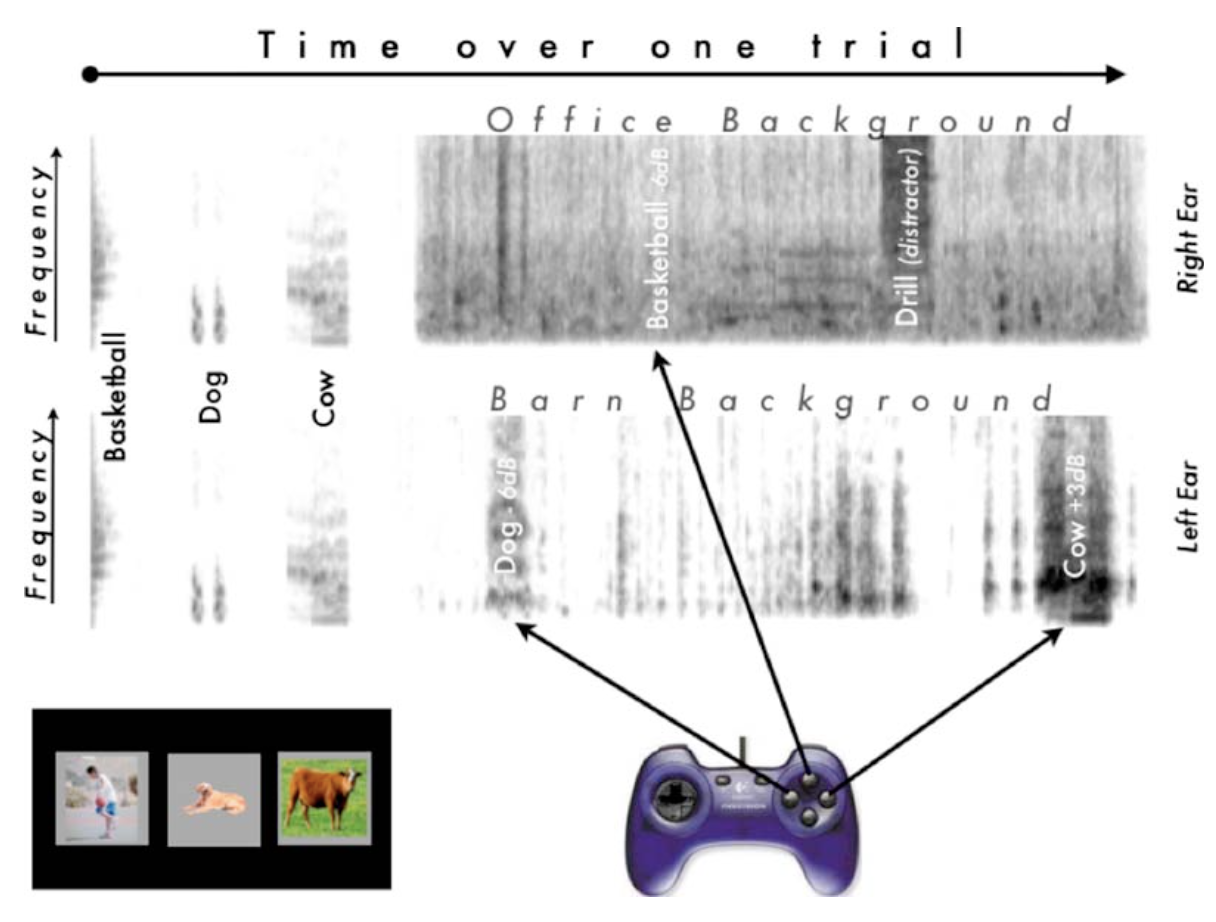
\includegraphics[width=0.65\linewidth]{figures/ENVASAparadigm} 

}

\caption{Schematic of the ENVASA experimental paradigm \autocite[taken from][]{Leech2009}}\label{fig:ENVASA}
\end{figure}

\hypertarget{celf-rs}{%
\subsubsection{CELF-RS}\label{celf-rs}}

The Recalling Sentences (RS) sub-test of the Clinical Evaluation of Language Fundamentals UK fifth edition \autocite[CELF-5-UK][]{HWiig2017} was administered to assess the listeners expressive language skills, measuring the ability to repeat in verbatim sentences with varying length and complexity. Standardised norms are available for children aged 5 to 16 years. The CELF-RS is simple and quick to administrate and has been shown to be a good psycholinguistic marker for children with Developmental Language Disorder (DLD) and to provide high levels of sensitivity and specificity \autocite{Conti-Ramsden2001}, thus making it a good screening tool. Scoring were marked by hand by the examiner as instructed by the test manual. The sentences were presented using a local MATLAB program via headphones using the same experimental equipment as listed above at a comfortable output level of 70~dB~HL. The sentences were spoken by a standard southern British English female and were recorded in a sound-treated recording booth at the SHaPS UCL laboratory, London. The task began with two practice sentences while the number of test items varied depending on the child's age and performance. No repetitions or feedback was given during the testing and the test was discontinued in case the child failed to score any points for four consecutive items. Age-scaled score were calculated based on the test norms with a mean score of 10 and SD of 3. Scaled scores within \(\pm\)~1~SD from the norms mean (between 8 to 12) are classified as average scores, whereas performance beyond \(\pm\)~1~SD are classified as above/below the average score. Thus, the cut-off for abnormally poor performance is a scaled score \(\leq\)~7.

\hypertarget{questionnaires}{%
\subsection{Questionnaires}\label{questionnaires}}

\hypertarget{medical-neurological-and-physiological-history}{%
\subsubsection*{Medical, Neurological, and Physiological History}\label{medical-neurological-and-physiological-history}}
\addcontentsline{toc}{subsubsection}{Medical, Neurological, and Physiological History}

\hypertarget{the-evaluation-of-childrens-listening-and-processing-skills-eclips}{%
\subsubsection*{The Evaluation of Children's Listening and Processing Skills (ECLiPS)}\label{the-evaluation-of-childrens-listening-and-processing-skills-eclips}}
\addcontentsline{toc}{subsubsection}{The Evaluation of Children's Listening and Processing Skills (ECLiPS)}

The ECLiPS questionnaire \autocite{Barry2014} comprises of 38 items where the users are asked to express their agreement simple statements about the child's listening and other related skills or behaviours using a five-point Likert scale (from ``strongly agree'' to ``strongly disagree''). The ECLiPS was design to identify listening and communication difficulties in children aged 6 to 11 years. Nonetheless, in their evaluation study, \textcite{Barry2014} found little to no age effect in many of the scale items, suggesting the testing age could be extended below and beyond the population used for the development. Based on factor analysis the items are grouped into five subcategories: 1. Speech \& Auditory Processing (SAP) assessing ability to interpret speech and non-speech input, 2. Environmental \& Auditory Sensitivity (EAS) estimating the ability to cope with environmentally challenging conditions, 3. Language, literacy \& laterality (L/L/L) assessing different abilities that are known to be coupled with language and literacy difficulties, 4. Memory \& Attention (M\&A) covering short-term and serial memory as well as attention, 5. Pragmatic \& Social skills (PSS) assessing pragmatic language or non-normative social behaviours. Aggregated measures were calculated for Listening (SAP, M\&A, \& PSS), Language (L/L/L \& M\&A), Social (PSS \& EAS), and a Total aggregate, calculated by taking the mean of scores across all the sub-scales. Individual age- and sex-scaled scores were computed using the test excel scorer. A score below the 10\(^{th}\) percentile (corresponding to a scale score of circa 6) is generally considered clinically significant.

\textbf{Discussion:} Correlation with CCC-2 sub-scales \autocite{Barry2014}: Overall, all the EClIPS sub scales shows strong correlation with most of the CCRM 10 sub-scales. Interestingly, PSS strongly correlates with all 10 CCC-2 sub-scales, suggesting that both tests taps into similar abilities.

\textbf{In the results:} compare scores with scores obtained by: \url{https://www.nature.com/articles/s41598-018-25316-9.pdf} and Moore et al.~2020 (Listening Difficulties in Children: Behaviour and Brain Activation Produced by Dichotic Listening of CV Syllables)

\hypertarget{the-childrens-communication-checklist-2nd-edition-ccc-2}{%
\subsubsection*{\texorpdfstring{The Children's Communication Checklist 2\(^{nd}\) edition (CCC-2)}{The Children's Communication Checklist 2\^{}\{nd\} edition (CCC-2)}}\label{the-childrens-communication-checklist-2nd-edition-ccc-2}}
\addcontentsline{toc}{subsubsection}{The Children's Communication Checklist 2\(^{nd}\) edition (CCC-2)}

Communication abilities were assessed using the Children's Communication Checklist second edition questionnaire \autocite[CCC-2;][]{Bishop2003} was completed by the child's parent/guardian. The CCC-2 was designed to screen communication problems in children aged 4 to 16 years and comprises of 70 checklist items each comprising of a behaviour statement like ``Mixes up words of similar meaning''. The respondents are asked to judge how often the behaviours occur using a four-point Likert rating scale: 0. \emph{less than once a week (or never)}, 1. \emph{at least once a week, but not every day}, 2. \emph{once or twice a day}, 3. \emph{several times (more than twice) a day (or always)}. The items are grouped into ten sub-scales of behaviours tapping into different skills (A. Speech, B. Syntax, C. Semantics, D. Coherence, E. Inappropriate initiation, F. Stereotyped language, G. Use of context, H. Non-verbal communication, I. Social relations, J. Interests). Taking the sum of scores for the sub-scales A to H are used to derive the General Communication Composite (GCC) which is used to identify clinically abnormal communication competence. A GCC score \textless{} 55 was found by \textcite{Norbury2005} to well separate between control and clinical groups, identifying children with scores at the bottom 10\%. Another composite (Social-Interaction Deviance Composite, SIDC) was taken by taking the difference in sum of scales E, H, I, and J from the sum of scales of A to D. Abnormal GCC (\textless~55) combined with a negative SIDC score has been shown to be indicative of an autistic spectrum disorder profile \autocite{Bishop2003}. The CCC-2 scaled and composite scores were computed using the test scorer. Data from one TD child out of forty four was excluded from the analysis due to inconsistent reports flagged by the test scorer.

\hypertarget{data-analysis}{%
\subsection{Data Analysis}\label{data-analysis}}

\hypertarget{age-scaled-scores}{%
\subsubsection{Age scaled scores}\label{age-scaled-scores}}

Age-independent scores were estimated using a linear regression model. The model was fitted per condition separately for each measure (ST-ASL, ST-CCRM, LiSNS-UK, SSN, \& ENVASA) and was based on the control group data only with the respective test raw measure score (e.g., SRdT, SRT or \%-correct) as the dependent variable and age as a predictor. A two-steps model comparison was performed to test the assumption that performance displays a monotonic linear relationship with age versus a non-monotonic (segmented) linear relationship. Extreme outliers were initially trimmed from the TD group to reduce noise in the data and to improve the models fit. In the first step, both models were computed and the best model was selected based on F-statistic model comparison using analysis of variance using \emph{anova()} function. Standard residuals were next calculated for each TD listener, based on the selected model prediction. Since age was included in the model, the standardised residuals are age-independent and are comparable to z-scores for data with normal distribution, with a mean and SD of approximately 0 and 1. Since the main goal of the study was to find a measure that is able to well separate between the APD group and the typically developed control group, individual differences and group differences were explored using a deviance analysis procedure proposed by \textcite{Ramus2003}. Abnormal scores were defined by a two-tailed deviance cut-off of \(\pm\)~1.96~SD from the TD group mean. Thus, circa 95\% of the normal population residuals are expected to be within the deviance range of \(\pm\)~1.96. Occasional occurrence of abnormal scores in the normal population is not unusual in behavioural measures. Therefore, since the prediction of the residuals is based on the control data, such outliers may skew the TD group true mean or SD and thus may introduce an error in the model prediction. Therefore, in the second step, additional TD outliers (with standardised residuals below/above TD mean \(\pm\)~1.96) were trimmed from the data and the two models were refitted and compared again. Finally, the model with the best fit was selected and was used to calculate the standardised residuals for all the listeners, including the trimmed TD observations and the APD group.

\hypertarget{statistical-analyses}{%
\subsubsection*{Statistical analyses}\label{statistical-analyses}}
\addcontentsline{toc}{subsubsection}{Statistical analyses}

All the statistical analyses were computed in R (version; REF). Residual analysis was performed separately for each measure to determine whether the data fulfils parametric methods assumptions of normal distribution using Shapiro-Wilk test \autocite[\emph{shapiro.test()},][]{RCore} and homogeneity of variance using Levene's test \autocite[\emph{leveneTest()};][]{carPackageR}. Consequently, statistical analyses for factorial design data that met these requirement was performed using a linear mixed-effects regression models (LMEMs). LMEM was fitted using the \emph{lmer()} function \autocite[lme4 package;][]{lme4PackageR}. Backward model selection procedure was applied to find the model that gives the best fit using a likelihood ratio test (\(\chi^2\)). Main effects and interaction terms were tested by comparing predictions of the full model to a reduced model where each fixed term was separately removed, starting with the interaction terms. When applicable, post-hoc paired comparison t-test was performed on the fitted model and included adjusted least-squared-mean for the random intercepts (subjects) using the \emph{lsmeans()} function from the emmeans R package \autocite{emmeansPackageR}. In addition, group differences for single parametric measures such as CELF-RS and CCC-2 total score were examined using \emph{boot.t.test()} function \autocite[MKinfer package;][]{MKinferPackageR} which performs independent-samples t-test with bootstrapping (n=9999).

Nonparamertic data was analysed using nparLD() function \autocite[nparLD package;][]{nparLDPackageR} which is a robust rank-based method for analysis of skewed data or with outliers or from a small sample size {[}see \autocite{Feys2016} for a good introduction for robust nonparametric techniques{]}. The function enables different types of nonparametric tests for factorial design data with repeated measures with variable between-/within-subjects factors. The results reported in the present study are based outputs of the ANOVA-type statistic test (ATS). Inspection of the ENVASA task age-independent z-scores revealed that the assumption of sphericity (Mauchly's test) was violated. Therefore, analysis was performed using \emph{npIntFactRep} package \autocite{npIntFactRepPackageR}, which is another robust aligned rank technique that enables sphericity correction (Greenhouse-Geisser). Post hoc comparison and group difference was examined using Wilcoxon rank-sum test with permutation (N=999999, independent two samples) which is a t-test equivalent for non-parametric data \autocite[\emph{coin::wilcox\_test()};][]{CoinPackageR}.

\hypertarget{results-3}{%
\section{Results}\label{results-3}}

\hypertarget{standard-audiometry-1}{%
\subsection{Standard audiometry}\label{standard-audiometry-1}}

Boxplots of listeners pure-tones detection thresholds measured at six octave frequency bands between 0.25 to 8~kHz and their corresponding PTAs are shown in Figure~\ref{fig:RegAud-fig}~A-B. Individuals PTAs were calculated separately for the right and left ear (PTA\(_{Right}\), PTA\(_{Left}\)) by taking the mean of thresholds at the frequency bands 0.5, 1, 2 and 4~kHz. In addition, PTA denotes the listeners grand-mean for PTAs in both ears, forming a single measure for the listeners hearing ability, and BE stands for the listeners PTA at the better-ear. Thresholds descriptives by frequency bands and ear split by the two groups is given in Table~\ref{tab:RegAud-Tab1}, whereas descriptives and statistics for PTAs and BE is given in Table~\ref{tab:RegAud-LMEMpost}.

\begin{figure}

{\centering \includegraphics[width=1\linewidth]{_main_files/figure-latex/RegAud-fig-1} 

}

\caption{Individual scores are indicated by circles. The boxes show the data interquartile range (25th-75th percentile) and the horizontal line indicate the median (i.e., 50th percentile). Values that fall within 1.5 times the interquartile range are indicated by the wiskers.}\label{fig:RegAud-fig}
\end{figure}

\begin{table}

\caption{\label{tab:RegAud-Tab1}Standard audiometry descriptives and test statistics for group differences tested using Wilcoxon rank-sum test for unpaired samples[note]. PTA$_{Right}$ and PTA$_{Left}$ were calculated by taking the individual mean for thresholds at 0.5, 1, 2 and 4 kHz in the respective ear. PTA denotes the listeners grand-mean for PTAs in both ears and BE represents the listeners PTA at the better-ear.}
\centering
\resizebox{\linewidth}{!}{
\begin{tabular}[t]{lcccccc|>{}ccccc}
\toprule
\multicolumn{2}{c}{ } & \multicolumn{5}{c}{APD} & \multicolumn{5}{c}{TD} \\
\cmidrule(l{3pt}r{3pt}){3-7} \cmidrule(l{3pt}r{3pt}){8-12}
Frequency & Ear & N & median & sd & min & max & N & median & sd & min & max\\
\midrule
250 & R & 20 & 10 & 3.73 & 0 & 15 & 23 & 5 & 3.95 & 0 & 15\\
500 & R & 20 & 5 & 4.94 & 0 & 15 & 23 & 10 & 4.49 & -5 & 15\\
1000 & R & 20 & 5 & 4.55 & -5 & 15 & 23 & 0 & 4.38 & -5 & 15\\
2000 & R & 20 & 5 & 3.97 & 0 & 15 & 23 & 5 & 3.76 & 0 & 10\\
4000 & R & 20 & 5 & 5.62 & -5 & 15 & 23 & 5 & 5.27 & -5 & 15\\
8000 & R & 20 & 10 & 5.36 & 0 & 20 & 23 & 10 & 8.29 & -5 & 30\\
\midrule
250 & L & 20 & 5 & 4.99 & 0 & 20 & 23 & 5 & 5.05 & -5 & 15\\
500 & L & 20 & 10 & 4.06 & 5 & 15 & 23 & 5 & 4.25 & -5 & 15\\
1000 & L & 20 & 5 & 3.84 & 0 & 15 & 23 & 0 & 3.99 & -5 & 10\\
2000 & L & 20 & 5 & 4.13 & 0 & 15 & 23 & 0 & 4.03 & -5 & 10\\
4000 & L & 20 & 5 & 5.95 & -5 & 15 & 23 & 5 & 6.07 & -5 & 20\\
8000 & L & 20 & 10 & 8.01 & 5 & 35 & 23 & 5 & 8.49 & -5 & 25\\
\bottomrule
\end{tabular}}
\end{table}

\colorbox[HTML]{CCCCFF}{Do the groups differ in their hearing abilities?}

Differences between the groups for detection thresholds across frequency bands and ears was statistically tested with a three-way 6~x~2~x~2 factorial design with repeated measures design. Inspection of the data by groups revealed that the assumption of normality and homoscedasticity were violated. Therefore, a non-parametric approach was adopted, using an rank-based ANOVA-type statistic test (ATS) with the \emph{nparLD()} function \autocite[nparLD package ;][]{nparLDPackageR}. The ATS test results are given in Table~\ref{tab:RegAud-TabnparLD}. There was no significant three-way or two-way interaction between the three factors Group, Frequency and Ear (p~\textgreater~0.05), albeit Group~x~Ear interaction reached significance level (p = 0.062). There was a significant main effect for group difference (p~\textless~0.05) as well as a highly significant difference in detection thresholds across frequencies (p~\textless~0.001), however no significant main effect for Ear was found (p=0.827).

\begin{table}

\caption{\label{tab:RegAud-TabnparLD}Statistical analysis for the effects of Frequency, Ear and Group as well as their interaction (6x2x2 factorial design with repeated measures) tested with a robust rank-based method for analysis of nonparametric data using nparLD package (Noguchi et al., 2012). Analysis was based on a f1-ld-f2 design ANOVA-type statistic (ATS) test, whereby f1 refers to an experimental design with a single between-subjects factor (Group) and f2 refers to two within-subjects factors (Frequency and Ear).}
\centering
\begin{tabular}[t]{llc>{}c}
\toprule
  & Statistic & df & p-value\\
\midrule
Group & 4.350 & 1.000 & \em{\textbf{0.037}}\\
Frequency & 26.856 & 3.970 & \em{\textbf{0.000}}\\
Ear & 0.048 & 1.000 & \em{0.827}\\
Group:Frequency & 0.990 & 3.970 & \em{0.411}\\
Ear:Frequency & 1.234 & 4.121 & \em{0.294}\\
Group:Ear & 3.493 & 1.000 & \em{0.062}\\
Group:Frequency:Ear & 1.716 & 4.121 & \em{0.141}\\
\bottomrule
\multicolumn{4}{l}{\textsuperscript{*} significant p-values (p < 0.05) are shown in bold.}\\
\end{tabular}
\end{table}

Differences in PTA and BE between the two groups were examined using a 4~x~2 LMEM model (parametric model assumptions were met). Detection measure (PTA\(_{Right}\), PTA\(_{Right}\), PTA and BE) and Group were set as fixed factors (reference levels: PTA\(_{Right}\) and TD group) and detection threshold (in dB~HL) as dependent variable, as well as a random intercept for subjects. A model with interaction term was found to give the best fit, showing a significant interaction between the calculated detection measure and Group {[}\(\chi^2\)(3)=12.27, p~\textless~0.05{]}. Post-hoc paired comparison t-test based on the fitted model was computed using lsmeans function from the emmeans R package {[}\textcite{emmeansPackageR}; see Table~\ref{tab:RegAud-LMEMpost}{]} revealed a significant difference between the groups for PTA's measured in the left ear (p~\textless~0.05), nonetheless, the magnitude of the difference between the two groups for PTA\(_{Left}\) (median difference of less than 5~dB) is rather small and clinically negligible, and thus is likely to occur due to sampling error. No significant difference was found in the remaining measures (all p's~\textgreater~0.05).



\begin{table}

\caption{\label{tab:RegAud-LMEMpost}Post-hoc paired comparison t-test for PTA x Group. The test was performed on the fitted LMEM model and included adjusted least-squared-mean for the random intercept (subjects) using lsmeans package (REF).}
\centering
\resizebox{\linewidth}{!}{
\begin{tabular}[t]{lccccc|>{}ccccc|>{}cccc>{}cc}
\toprule
\multicolumn{1}{c}{ } & \multicolumn{5}{c}{APD} & \multicolumn{5}{c}{TD} & \multicolumn{6}{c}{post-hoc paired t-test} \\
\cmidrule(l{3pt}r{3pt}){2-6} \cmidrule(l{3pt}r{3pt}){7-11} \cmidrule(l{3pt}r{3pt}){12-17}
 & N & median & sd & min & max & N & median & sd & min & max & Estimate & SE & Df & t-value & p-value & 95\%-CI\\
\midrule
PTA$_{Right}$ & 20 & 4.38 & 3.78 & -1.25 & 12.50 & 23 & 3.75 & 3.16 & -2.5 & 11.25 & 0.799 & 0.942 & 59.762 & 0.848 & \em{0.4} & -1.09 - 2.68\\
PTA$_{Left}$ & 20 & 5.00 & 3.04 & 0.00 & 11.25 & 23 & 2.50 & 3.01 & -2.5 & 8.75 & 2.682 & 0.942 & 59.762 & 2.846 & \em{\textbf{0.006}} & 0.8 - 4.57\\
PTA & 20 & 5.31 & 2.92 & 0.62 & 10.62 & 23 & 3.75 & 2.87 & -2.5 & 10.00 & 1.740 & 0.942 & 59.762 & 1.846 & \em{0.07} & -0.15 - 3.62\\
BE & 20 & 3.75 & 3.17 & -1.25 & 8.75 & 23 & 2.50 & 2.68 & -2.5 & 8.75 & 1.242 & 0.942 & 59.762 & 1.318 & \em{0.193} & -0.64 - 3.13\\
\bottomrule
\multicolumn{17}{l}{\textsuperscript{*} significant p-values (p < 0.05) are shown in bold.}\\
\end{tabular}}
\end{table}

\hypertarget{ehfa}{%
\subsection{EHFA}\label{ehfa}}

The listeners pure-tone detection thresholds measured at the octave frequency bands 8, 11 and 16~kHz are plotted in Figure~\ref{fig:EHF} separately for the left and the right ear. The thin black lines represents individuals' thresholds in the APD group and the group mean is marked by the bold black line. The shaded grey area represents the TD group thresholds range and the white line represents their mean at each frequency. A comparison of the group means reveals relatively small differences in thresholds between the groups, with a relatively larger difference in the left ear, where APD thresholds at 11 and 16~kHz were on average 5 dB higher (i.e., poorer).

\begin{figure}

{\centering \includegraphics[width=0.85\linewidth]{_main_files/figure-latex/EHF-1} 

}

\caption{APD listeners pure-tone detection thresholds for extended high-frequency bands measured in the left and the right ear. The thin black lines represents the individual thresholds in the APD group and the group mean is marked by the bold black line. The shaded grey area represents the TD group threshold range and the white line represents the group mean at each frequency.}\label{fig:EHF}
\end{figure}

Boxplots of the listeners thresholds by frequency and ear as well as their calculated PTA's and BE are shown in Figure~\ref{fig:EHF-Boxplot} A-B. Descriptives of the groups detection thresholds is given in Table~\ref{tab:EHF-tab}.

\begin{figure}

{\centering \includegraphics[width=1\linewidth]{_main_files/figure-latex/EHF-Boxplot-1} 

}

\caption{Boxplots for the pure-tone detection thresholds measured with ER10x at the extended high-frequency bands split by ear and groups (A). Boxplots of the groups averaged PTA collapsed by ear as well as averaged across both ears and the listeners better-ear is depicted in figure B. Individual scores are indicated by circles. The boxes show the data interquartile range (25th-75th percentile) and the horizontal line indicate the median (i.e., 50th percentile). Values that fall within 1.5 times the interquartile range are indicated by the wiskers.}\label{fig:EHF-Boxplot}
\end{figure}

\begin{table}

\caption{\label{tab:EHF-tab}Extended high frequency detection thresholds descriptive collapsed by group.}
\centering
\resizebox{\linewidth}{!}{
\begin{tabular}[t]{lcccccc|>{}ccccc}
\toprule
\multicolumn{2}{c}{ } & \multicolumn{5}{c}{APD} & \multicolumn{5}{c}{TD} \\
\cmidrule(l{3pt}r{3pt}){3-7} \cmidrule(l{3pt}r{3pt}){8-12}
 & Ear & N & median & sd & min & max & N & median & sd & min & max\\
\midrule
\addlinespace[0.3em]
\multicolumn{12}{l}{\textbf{octave frequency bands}}\\
\hspace{1em}8000 & R & 18 & 12.5 & 7.28 & 5.0 & 30 & 21 & 10.0 & 8.42 & 0 & 35\\
\hspace{1em}11000 & R & 18 & 10.0 & 11.48 & 0.0 & 45 & 21 & 10.0 & 11.97 & 0 & 45\\
\hspace{1em}16000 & R & 18 & 2.5 & 10.04 & 0.0 & 30 & 21 & 0.0 & 10.51 & 0 & 35\\
\hspace{1em}8000 & L & 18 & 15.0 & 7.48 & 0.0 & 30 & 21 & 15.0 & 6.64 & 0 & 25\\
\hspace{1em}11000 & L & 18 & 10.0 & 11.99 & 5.0 & 45 & 21 & 10.0 & 9.55 & 0 & 40\\
\hspace{1em}16000 & L & 18 & 5.0 & 14.12 & 0.0 & 40 & 21 & 0.0 & 8.11 & 0 & 25\\
\addlinespace[0.3em]
\multicolumn{12}{l}{\textbf{PTAs and better-ear}}\\
\hspace{1em}PTA$_{Right}$ & R & 18 & 10.0 & 8.50 & 0.0 & 25 & 21 & 5.0 & 10.18 & 0 & 35\\
\hspace{1em}PTA$_{Left}$ & L & 18 & 10.0 & 10.68 & 0.0 & 40 & 21 & 10.0 & 7.57 & 0 & 25\\
\hspace{1em}PTA &  & 18 & 10.0 & 8.80 & 2.5 & 30 & 21 & 7.5 & 8.35 & 0 & 35\\
\hspace{1em}BE &  & 18 & 5.0 & 7.78 & 0.0 & 25 & 21 & 5.0 & 7.44 & 0 & 25\\
\bottomrule
\end{tabular}}
\end{table}

\colorbox[HTML]{CCCCFF}{Difference between groups}

Difference in thresholds between the two groups across frequencies (8, 11, \& 16~kHz) and ears (left/right) were examined for a 3~x~2~x~2 repeated measures factorial design. Inspection of parametric model assumptions revealed that the groups data violated the assumption of normality and homoscedasticity. Therefore, the exact same nonparametric procedure as used for the standard audiometry was performed using nparLD package (see section ??). The ATS ANOVA-type test given in Table~\ref{tab:EHF-TabnparLD} found no significant three-way nor two way interaction between the different factors. There was however a highly significant difference in thresholds between the three frequency bands (p~\textless~0.001), whereas no significant main effect for Group or Ear was found.

\begin{table}

\caption{\label{tab:EHF-TabnparLD}EHF statistical analysis for the effects of Frequency, Ear and Group as well as their interaction (3x2x2 factorial design with repeated measures) tested with a robust rank-based method for analysis of nonparametric data using nparLD package (Noguchi et al., 2012). Analysis was based on a f1-ld-f2 design ANOVA-type statistic (ATS) test, whereby f1 refers to an experimental design with a single between-subjects factor (Group) and f2 refers to two within-subjects factors (Frequency and Ear).}
\centering
\begin{tabular}[t]{lcc>{}c}
\toprule
  & Statistic & df & p-value\\
\midrule
Group & 1.323 & 1.000 & \em{0.25}\\
Frequency & 22.019 & 1.717 & \em{\textbf{0.000}}\\
Ear & 0.395 & 1.000 & \em{0.53}\\
Group:Frequency & 1.036 & 1.717 & \em{0.346}\\
Ear:Frequency & 0.427 & 1.969 & \em{0.649}\\
Group:Ear & 0.348 & 1.000 & \em{0.555}\\
Group:Frequency:Ear & 0.220 & 1.969 & \em{0.799}\\
\bottomrule
\multicolumn{4}{l}{\textsuperscript{*} significant p-values (p < 0.05) are shown in bold.}\\
\end{tabular}
\end{table}

Similarly, additional nonparametric 4~x~2 factorial design model was used to examine the difference between the two groups for the four combined threshold measures (PTA\(_{Right}\), PTA\(_{Left}\), PTA, and BE). The nparLD ATS test found no significant two-way interaction between Group and Measure nor a main effect of groups, while there was a significant main effect of measure (see Table~\ref{tab:EHF-PTATabnparLD}).

\begin{table}

\caption{\label{tab:EHF-PTATabnparLD}EHF statistical analysis for the effects of the listeners calculated summary measures (PTA$_{Right}$, PTA$_{Left}$, PTA, and BE) and Group as well as their interaction (4x2 factorial design with repeated measures) tested with a robust rank-based method for analysis of nonparametric data using nparLD package (Noguchi et al., 2012). Analysis was based on a f1-ld-f1 design ANOVA-type statistic (ATS) test, whereby f1 refers to an experimental design with a single between-subjects factor (Group) and a single within-subjects factor (Measure).}
\centering
\begin{tabular}[t]{lcc>{}c}
\toprule
  & Statistic & df & p-value\\
\midrule
Group & 1.189 & 1.000 & \em{0.275}\\
Measure & 7.429 & 1.379 & \em{\textbf{0.003}}\\
Group:Measure & 0.089 & 1.379 & \em{0.843}\\
\bottomrule
\multicolumn{4}{l}{\textsuperscript{*} significant p-values (p < 0.05) are shown in}\\
\multicolumn{4}{l}{bold.}\\
\end{tabular}
\end{table}

\hypertarget{st}{%
\subsection{ST}\label{st}}

\hypertarget{outliers-missing-data}{%
\subsubsection*{Outliers \& missing data}\label{outliers-missing-data}}
\addcontentsline{toc}{subsubsection}{Outliers \& missing data}

As a first step, the listeners adaptive track and psychometric functions (PF) were manually inspected for abnormalities. The proportion of correct keywords within the final test trials (LevsPC) was calculated as a measure describing the success of the adaptive procedure. Since the adaptive procedure was set to yield 50\%-correct, a successful procedure is expected to be within the 50\% range. A binomial statistical test was applied to identify observations that significantly differ from 50\%. Observations with LevsPC~\(\leq\)~35\% were flagged as possible outliers and were further inspected (see bottom panel of Figures~\ref{fig:ST-ASLLevsPC}-\ref{fig:ST-CCRMLevsPC}). Interestingly, the majority of the flagged outliers belonged to the CCRM data with 29 observations out of 258 (6 conditions x 43 listeners), whereas only 3 observations out of 215 (5 conditions x 43 listeners) were flagged for data measured with the ASL speech material.

As expected, most of the identified cases in both materials were for observations measured with the more demanding conditions with speech distractors. In five cases (2 ASL; 3 CCRM) we were able to confidently determine that the listener's true score was near to ceiling, and thus these observations were set to the maximum DC (0.97). In other cases it was not possible to confidently determine the true SRdT, either because the procedure ended after reaching the maximum number or trials before a minimum number of test reversals was obtained (CCRM~=~1; ASL~=~2), or due to aberrant adaptive tracks (CCRM~=~5). Since all these cases belonged to more challenging test conditions with speech distractors, it is very likely that the children's true score is at celling. Thus, to account for that, rather than removing these observations, which will consequently reduce the statistical power and may won't capture the true performance in the group, they were set to a DC of 1, which is above the task's upper DC limit of 0.97.

\begin{figure}
\includegraphics[width=1\linewidth]{_main_files/figure-latex/ST-ASLLevsPC-1} \caption{ST raw data: frequency of possible outliers for observations with LevsPC $\leq$ 35\%. LevsPC denotes the proportion of correct keywords within the final test trials.}\label{fig:ST-ASLLevsPC}
\end{figure}

\hypertarget{srdts-by-age}{%
\subsubsection*{SRdTs by age}\label{srdts-by-age}}
\addcontentsline{toc}{subsubsection}{SRdTs by age}

Since the present study sample comprised of young children from different age groups from circa 7 to 13 years, developmental age effect was expected, whereby performance was expected to improve with an increasing age due to different maturity effects. This is illustrated by the scatterplots and linear regression lines plotted in Figure~\ref{fig:ST-Age}~A-B for the listeners SRdTs obtained across the different test conditions and speech material (ASL/CCRM) split by groups. Note that smaller SRdT indicates better performance. Age effect was tested against the TD group only since this group is more heterogeneous and thus expected do display smaller variability than in the APD group. Nonetheless, despite the larger spread in the APD group, the group showed similar trend in performance, albeit shifted towards higher SRdTs (i.e., poorer performance). The TD regression lines were determined based on a model comparison and outliers trimming procedure described in section ??? to improve model prediction. Regular regression lines were found to be the most parsimonious in describing the relationship between the TD children performance and their age. This was the case in all test conditions but the MDR\_F distractor in the ASL material, where a segmented line was found to give the best fit. MDR\_F segmented line indicated that DC improved with age by circa 0.1 per year until reaching a plateau at the age of 9.5 years.

\begin{figure}[h]

{\centering \includegraphics[width=1\linewidth]{_main_files/figure-latex/ST-Age-1} 

}

\caption{Scatterplot and linear regression lines for the listeners SRdTs measured with the switching task with the ASL (A) and CCRM speech material (B) as a function of age. Corresponding regression coefficients and statistics is provided for TD group only. Red indicates data from the APD group and cyan indicates data from the TD control group. Data for normal hearing adults taken from Chapter 2 is shown in the boxplots as a reference.}\label{fig:ST-Age}
\end{figure}

Looking at Figure~\ref{fig:ST-Age}~A-B, it is noticeable that children in both groups showed a larger decrement in performance when presented with speech distractors. The regression lines indicates that the improvement in performance by age was more prominent for speech distractors, with relatively steeper slopes (at least twice as steep) than for the non-speech distractor (AMSSN) or for conditions without a distractor. Furthermore, as expected, CCRM sentences were more intelligible, with performance shifted towards lower DC range (i.e., more difficult) relative to performance for the ASL speech material. \colorbox[HTML]{CCCCFF}{\emph{Belongs to discussion?}} The improved intelligibility in the CCRM material is amongst others due to the more simple speech material, the reduced confusion between the target sentences and the connected speech distractors as well as the restricted alternative responses of the CCRM matrix-based sentences.

A closer look at the linear lines shows several interesting trends. The non-speech AMSSN distractor showed to have little-to-no effect on performance, at least in the TD group, where performance was fairly similar to performance in the Quiet conditions. Introducing alternations (as in Quiet-NoAlt vs.~Quiet-Alt), seems to hinder intelligibility in both groups, however the effect is relatively small and may not be significant due to the large spread in the APD group. When comparing the regression lines, there appears to be a relatively larger separation between the groups for data measured with the CCRM material, especially for AMSSN, but also for the speech distractors. However, it is possible that the APD regression lines do not reflect the true population due to the large spread in performance and the small sample size and thus any interpretation should be taken with a pinch of salt. Another interesting observation is that the children showed little-to-no \emph{masking-release} for speech spoken in an unfamiliar language (MDR\_F) when compared with a distractor spoken in English (ENG\_F). This is in agreement with findings in the adults study in Chapter~\ref{Chpt2}. Lastly, it is apparent from the figure that performance for CCRM\_F distractor was near-to-ceiling for some children, mostly among the APD group.

An exploratory comparison between between the children's data measured in the present study with data measured across young NH adults collected in Chapter~\ref{Chpt2} further highlight the strong developmental trend, with SRdTs still not entirely ``adult-like'' even at the age of 13 years, especially for speech distractos (see boxplots in Figure~\ref{fig:ST-Age}~A-B). The children in both groups seems to be markedly susceptible to competing CCRM sentences or familiar/unfamiliar speech presented with ASL sentences, with performance at the age of 12 years still largely differing from those obtained by the adults. On the other hand, by the age of 12 years, the TD children reached near to ``adult-like'' performance when CCRM target sentences were presented with with ENG\_F speech distractor or when ASL sentences were presented with AMSSN distractor.

Next, age effect was evaluated using LMEM, with Condition, Material (ASL/CCRM) and Age as fixed factors, SRdT as dependent variable and a random intercept for subjects (reference levels: Condition = Quiet-NoAlt; Material = ASL).
Note that data for CCRM\_F was excluded from the model since it was only measured for the CCRM material \colorbox[HTML]{CCCCFF}{(a separate model for CCRM found significant Condition x Age interaction)}. Additional random intercept for APD siblings resulted in singular fit an was thus removed from the final mode. A model without three-way interaction between Condition, Material and Age was found to give the best fit (see Table~\ref{tab:ST-AgeLMEM}). Parametric assumption inspection of normal distribution was met, whereas the assumption of homogeneity of variance was marginal (\emph{p=0.04}). Model comparison revealed a highly significant two-way interaction between Condition~x~Age (p~\textless~0.001) as well as a marginal two-way interaction between Condition~x~Material and Material~x~Age (p~=~0.052) which further support the trends seen in the scatterplots.

\textcolor{red}{The significant Material x Age interaction indicates that the developmental trend is different between the two speech materials, with larger age effect (i.e., steeper slopes) for the ASL than for the CCRM sentences(?????). [the LMEM summary gives an estimate for materialCCRM:Age of 0.014 (ASL is the reference level). Does that mean that the ASL sentences mean improvement per 1 year was 0.014 larger than for the CCRM material? I'm not too sure how to interpret this..]} Furthermore, the significant Condition~x~Material interaction implies that performance in the different test conditions differed between the two speech materials. A post-hoc t-test comparison based on the fitted model (see Table~\ref{tab:ST-AgeLMEMpost}), revealed a highly significant difference in performance between the speech materials across all five test conditions (all p's \textless~0.001). The estimated mean difference between the contrast pairs ranged between +0.18 to +0.27, hence, the CCRM speech material was significantly more intelligible than the ASL material, across all test conditions.

Lastly, the highly significant Condition~x~Age interaction supports the observation in Figure~\ref{fig:ST-Age}~A-B, that the magnitude of the age effect was different across the test conditions. These findings raises the following questions -- do all the conditions show a significant age effect? Moreover, since the effect of age is not the same across the test conditions, which conditions showed the largest age effect? One possible way to tackle these questions is to compare the separate regression models using F-statistics. Nonetheless, due to the small sample-size and the large number of paired comparisons, such test lacks a statistical power and the results may not reflect the true effect in a larger sample. The TD group regression model's R\(^{2}\) and p-values are given in the bottom part of Figure A and B. The ASL model's p-value indicated a highly significant age effect for ENG\_F, MDR\_F and Quiet-NoAlt condition and a marginal effect for AMSSN (p=0.048), whereas no significant age effect was found for Quiet-Alt (p=0.168). As for the CCRM material, there was a highly significant age effect for ENG\_F and a marginal effect for the Quiet-Alt condition (p=0.058) and for CCRM\_F condition (p=0.05) which is not included in the LMEM model, whilst no significant age effect was found for Quiet-NoAlt, AMSSN and MDR\_F conditions. Furthermore, age was found to be a better predictor (i.e., accounting for larger variance in SRdT) for conditions with speech distractors, with R\(^{2}\) ranging between 32\% to 72\% for the ASL material and about 12\% to 29\% for the CCRM material. A comparison between the test conditions regression line slopes fitted for the CCRM (x-axis) and ASL speech material (y-axis) is depicted in Figure~\ref{fig:ST-AgeSlopes}. A possible pattern emerges from the figure, where slopes for the quiet and non-speech conditions are fairly similar across the two speech material (indicated by their proximity to the diagonal line), while, differences between the slopes are relatively larger for speech distractors, in particularly for MDR\_F where the slope for the ASL material (-0.13) is about six times steeper than the slope for the CCRM material (-0.02).

\begin{table}

\caption{\label{tab:ST-AgeLMEM}ST - age effect: LMEM for SRdTs measured across condition, speech material and age as fixed factors and a random intercept for subjects. Reference levels: Condition = Quiet-NoAlt, Group = APD, Material = ASL). Note: only data measured with the control group following outliers trimming was included (trimmed TD). }
\centering
\begin{tabular}[t]{>{\raggedright\arraybackslash}p{8cm}cc>{}c}
\toprule
\multicolumn{4}{l}{SRdT \textasciitilde{} Condition + Material + Age} \\
\multicolumn{4}{c}{+ Condition:Material + Condition:Age + Material:Age + (1 | Subjects)} \\
\cmidrule(l{3pt}r{3pt}){1-4}
Main effects & Df & $\chi^{2}$ & p\\
\midrule
Condition:Material & 4 & 9.385 & \em{\textbf{0.052}}\\
Condition:Age & 4 & 14.919 & \em{\textbf{0.005}}\\
Material:Age & 1 & 3.786 & \em{\textbf{0.052}}\\
\bottomrule
\multicolumn{4}{l}{\textsuperscript{*} significant p-values (p < 0.05) are shown in bold.}\\
\end{tabular}
\end{table}



\begin{table}

\caption{\label{tab:ST-AgeLMEMpost}ST - age effect: Post-hoc paired comparison t-test for Condition x Material two-way interaction. The test was performed on the fitted LMEM model and included adjusted least-squared-mean for the random intercept (subjects) using lsmeans package \autocite[emmeans package;][]{emmeansPackageR}.}
\centering
\resizebox{\linewidth}{!}{
\begin{tabular}[t]{lcccc>{}cc}
\toprule
Contrasts & Estimate & SE & Df & t-value & p-value & 95\%-CI\\
\midrule
(Quiet-NoAlt ASL) - (Quiet-NoAlt CCRM) & 0.19 & 0.03 & 216.45 & 7.62 & \em{\textbf{< 0.001}} & 0.14 - 0.24\\
(Quiet-Alt ASL) - (Quiet-Alt CCRM) & 0.20 & 0.03 & 216.21 & 8.01 & \em{\textbf{< 0.001}} & 0.15 - 0.25\\
(AMSSN-Alt ASL) - (AMSSN-Alt CCRM) & 0.18 & 0.03 & 216.25 & 7.37 & \em{\textbf{< 0.001}} & 0.14 - 0.23\\
(MDR\_F-Alt ASL) - (MDR\_F-Alt CCRM) & 0.24 & 0.03 & 216.21 & 9.66 & \em{\textbf{< 0.001}} & 0.19 - 0.29\\
(ENG\_F-Alt ASL) - (ENG\_F-Alt CCRM) & 0.27 & 0.03 & 216.21 & 10.90 & \em{\textbf{< 0.001}} & 0.22 - 0.32\\
\bottomrule
\multicolumn{7}{l}{\textsuperscript{*} significant p-values (p < 0.05) are shown in bold.}\\
\end{tabular}}
\end{table}

\begin{figure}

{\centering \includegraphics[width=0.6\linewidth]{_main_files/figure-latex/ST-AgeSlopes-1} 

}

\caption{ST - age effect: A comarison beteween the regression lines slopes fitted for the CCRM (x-axis) and ASL speech material (y-axis) in the switching task. The different test conditions are represented by the different symbols given in the legend. The diagonal line represents an optimal agreement between the speech materials. Observations falling below the line indicate steeper slope for the ASL material than compared with the CCRM material.}\label{fig:ST-AgeSlopes}
\end{figure}

\hypertarget{age-independent-z-scores}{%
\subsubsection*{Age-independent z-scores}\label{age-independent-z-scores}}
\addcontentsline{toc}{subsubsection}{Age-independent z-scores}

\colorbox[HTML]{CCCCFF}{\emph{Boxplots \& abnormal scores by conditions}}

Age-independent standardised residuals z-scores were calculated based on a model prediction based the TD group data using a multiple-case study approach (\textcite{Ramus2003}; see section ??? for more details). Descriptive statistics for the listeners z-scores is giving in Table~\ref{tab:ST-Tab}. Additional boxplots are shown in Figure~\ref{fig:ST-z}~A-B, for the ASL and CCRM speech material respectively. Scores were calculated separately for each test condition, with better performance indicated by lower z-score. The grey area marks the two-tailed 1.96 deviance cut-off for abnormal score from the control group mean (z~\(\approx\)~0), where only about 5\% of the normal population is expected to score below/above it. Overall, APD children performance was noticeably poorer in both test material, with higher median z-scores than compared with the TD children. The next paragraphs will cover the examination and statistical analysis of the individuals and group differences separately for each speech material.

\begin{figure}

{\centering \includegraphics[width=1\linewidth]{_main_files/figure-latex/ST-z-1} 

}

\caption{ST: Boxplots of the listeners age-independent standardised residuals for data measured with the ASL (A) and the CCRM speech material (B). Residuals were calculated seperately for each condition and are based on a model predicton for TD group only. The grey area represents the deviance cut-off for abnormal score (SD $\pm$ 1.96 below/above the TD mean), where about 95\% of the normal population is e expected to lay within. The dashed line represents the theorethical TD group mean (z = 0). Individual scores are indicated by circles. The boxes show the data interquartile range (25th-75th percentile) and the horizontal line indicate the median (i.e., 50th percentile). Values that fall within 1.5 times the interquartile range are indicated by the wiskers.}\label{fig:ST-z}
\end{figure}

\begin{table}

\caption{\label{tab:ST-Tab}ST: Descriptives for standardised residuals (z-scores) calculated for data measured with the ASL and CCRM speech material. 'abnormal' is referred to the percentage of abnormal score, defined as z-score > 1.96.}
\centering
\resizebox{\linewidth}{!}{
\begin{tabular}[t]{lcccccc|>{}ccccll}
\toprule
\multicolumn{1}{c}{ } & \multicolumn{6}{c}{APD} & \multicolumn{6}{c}{TD} \\
\cmidrule(l{3pt}r{3pt}){2-7} \cmidrule(l{3pt}r{3pt}){8-13}
 & N & median & sd & min & max & abnormal & N & median & sd & min & max & abnormal\\
\midrule
\addlinespace[0.3em]
\multicolumn{13}{l}{\textbf{ASL}}\\
\hspace{1em}Quiet-NoAlt & 20 & 1.81 & 1.39 & -0.76 & 3.74 & 45.00\% & 23 & 0.00 & 1.96 & -1.69 & 6.05 & 13.04\% (4.76\%)\\
\hspace{1em}Quiet-Alt & 20 & 0.29 & 0.87 & -0.79 & 2.12 & 10.00\% & 23 & -0.13 & 1.46 & -1.72 & 5.27 & 4.35\% (0.00\%)\\
\hspace{1em}AMSSN-Alt & 20 & 1.79 & 1.45 & -0.82 & 4.50 & 50.00\% & 23 & 0.10 & 2.35 & -2.18 & 9.04 & 13.04\% (9.52\%)\\
\hspace{1em}MDR\_F-Alt & 20 & 0.99 & 1.75 & -1.31 & 5.37 & 40.00\% & 23 & -0.13 & 1.11 & -1.44 & 2.91 & 8.70\% (4.76\%)\\
\hspace{1em}ENG\_F-Alt & 20 & 0.90 & 1.53 & -2.96 & 3.09 & 20.00\% & 23 & 0.12 & 1.55 & -4.44 & 1.75 & 0.00\% (0.00\%)\\
\addlinespace[0.3em]
\multicolumn{13}{l}{\textbf{CCRM}}\\
\hspace{1em}Quiet-NoAlt & 20 & 0.36 & 1.75 & -1.73 & 5.70 & 20.00\% & 23 & 0.38 & 1.57 & -1.92 & 5.72 & 8.70\% (0.00\%)\\
\hspace{1em}Quiet-Alt & 20 & 0.47 & 1.23 & -1.66 & 3.58 & 15.00\% & 23 & -0.08 & 1.19 & -1.68 & 3.44 & 4.35\% (0.00\%)\\
\hspace{1em}AMSSN-Alt & 20 & 1.62 & 2.03 & -1.39 & 7.95 & 40.00\% & 23 & -0.28 & 1.09 & -1.38 & 2.50 & 4.35\% (0.00\%)\\
\hspace{1em}MDR\_F-Alt & 20 & 0.86 & 1.40 & -1.12 & 4.06 & 25.00\% & 23 & 0.28 & 1.11 & -1.87 & 2.77 & 4.35\% (0.00\%)\\
\hspace{1em}ENG\_F-Alt & 20 & 1.05 & 1.22 & -0.80 & 3.25 & 20.00\% & 23 & 0.26 & 1.14 & -1.80 & 2.99 & 4.35\% (0.00\%)\\
\hspace{1em}CCRM\_F-Alt & 20 & 1.11 & 0.89 & -1.59 & 2.24 & 10.00\% & 23 & 0.24 & 0.98 & -1.76 & 1.47 & 0.00\% (0.00\%)\\
\bottomrule
\multicolumn{13}{l}{\textsuperscript{} abnormal: the percentage of abnormal score, defined as z-score > 1.96.}\\
\multicolumn{13}{l}{\textsuperscript{} Percentage in brackets were accounted for observations that were trimmed during the z-score calculation procedure.}\\
\end{tabular}}
\end{table}

\hypertarget{asl-corpus}{%
\paragraph*{ASL corpus}\label{asl-corpus}}
\addcontentsline{toc}{paragraph}{ASL corpus}

Surprisingly, a comparison of the groups averaged z-score reveals that the non-switched Quiet condition (Quiet-NoAlt) and the switched condition with non-speech distractor (AMSSN) yielded the largest separation between the groups, with APD median z-score of 1.81 and 1.79, respectively, laying just within the norms upper limit. Performance of the APD children was also noticeably poorer for conditions with speech distractors (MDR\_F and ENG\_F), with median z-score of circa 1, whereas performance for Quiet-Alt condition was fairly similar between the groups.

Within the APD group AMSSN, Quiet-NoAlt and MDR\_F resulted in the highest proportion of abnormal scores\footnote{Focusing on future clinical viability of the task, we were only interested in identifying children with clinically poor performance. Thus, abnormal score was defined as a one-tailed deviance cut-off of z-score \textgreater{} 1.96, within which circa 97.5\% of the normal population is expected to lay.}. Surprisingly, AMSSN distractor yielded the highest proportion of abnormal scores, where half of the APD children fell outside the norm (20/10, 50\%). Followed by the non-switched condition Quiet-NoAlt, where paradoxically and against our expectation 45\% of the APD group (9/20) had abnormally poor score, whereas only 10\% (2/20) had abnormal score in the switched condition Quiet-Alt. Another interesting finding was that the APD children did not benefit from a release of masking for a speech distractor spoken in an unfamiliar language (MDR\_F) as opposed to a familiar speech spoken in English (ENG\_F), with median scores very similar in both conditions. This sits well with our previous findings with adults where adults showed no benefit for MDR\_F speech masker (see chapter ???). Moreover, while the overall performance was similar in the two conditions, the percentage of abnormal score was twice as large for MDR\_F condition (8/20, 40\%) than for ENG\_F condition (4/20, 20\%). The proportion of abnormal scores amongst the TD group ranged between 0\% to 13\% (mean~=~7.8\%), which is relatively higher than expected in the normal population. Nonetheless, when taking into account TD observations that were trimmed during the z-score calculation procedure, the proportion of abnormal scores are smaller, ranging between 0\% to 9.5\% (mean~=~3.8\%), which corroborate fairly well with the theoretical probability of 2.5\% (one-tailed).

\hypertarget{ccrm-corpus}{%
\paragraph*{CCRM corpus}\label{ccrm-corpus}}
\addcontentsline{toc}{paragraph}{CCRM corpus}

Figure \ref{fig:ST-z}~B reveals a similar trend for the CCRM sentences, nonetheless with a more modest differences between the two groups. Again, AMSSN yielded the largest separation between the groups, where 40\% (8/20) of the APD children obtained an abnormal score and with a median score of 1.62, which is relatively close to the +1.96 upper deviance cut-off. In comparison, only 4.3\% of the TD children (1/23) had abnormal performance for AMSSN condition. The APD group median score for the speech distractors was approximately 1 (range: 0.86-1.11), however the proportion of abnormal APD children was noticeably smaller than seen for AMSSN, with 25\% (5/20) for MDR\_F, 20\% (4/20) for ENG\_F, and only 10\% (2/20) for CCRM\_F distractor. Lastly, in contrast to the ASL material, performance for the CCRM sentences presented in quiet were relatively better without switching (NoAlt) than with switching (Alt). Nonetheless, the spread in performance for the non-switched condition was larger. The percentage of abnormal scores in the TD group were relatively low ranging between 0 to 8.7\% (mean~=~4.3\%) and were at 0\% across all conditions when TD observations that were trimmed as part of the z-score calculation procedure were accounted for.

\colorbox[HTML]{CCCCFF}{\emph{nparLD() full 2x2x5 model}}

A three-way 2~x~2~x~5 factorial design model with repeated measures was used to test the main effects of Group, Condition, and Material as well as their interaction on performance in the task (with z-scores as dependent variable). Note that the model did not include the CCRM test condition with CCRM-type sentences as distractor (CCRM\_F) since there was no comparable condition in the ASL speech material. Inspection of the data revealed that the assumption of normal distribution was rejected for data measured with both speech material. Furthermore, homogeneity of the variance in the APD group was rejected for the ASL corpus. Thus, due to the small sample size and the incomplete fulfilment of parametric statistical methods assumptions, a non-parametric approach was adopted. This was tested with a rank-based ANOVA-type statistic test (ATS) using the \emph{nparLD()} function \autocite[nparLD package;][]{nparLDPackageR}. The analysis was based on a f2-ld-f1 design ATS test, whereby f2 refers to an experimental design with two between-subjects factors (Group \& Material) and f1 refers to a single within-subjects factor (Condition).The test results are given in Table~\ref{tab:ST-Tab-nparLD}. No significant three-way or two-way interactions were found (Group~x Condition~x~Material, Group~x~Material, Material~x~Condition, and Group~x~Condition; all p's~\textgreater~0.05), while there was a highly significant main effect of Group (p~\textless{} 0.0001) and a strong main effect of Condition (p~\textless{} 0.001). Despite some evidence for better performance in the CCRM material, the main effect of Material was not significant (p~=~0.62). Furthermore, in spite of some apparent differences in performance between the two groups across the different test conditions, these differences were found to be insignificant based on the Group~x~Condition two-way interaction.

\colorbox[HTML]{CCCCFF}{\emph{additional model for CCRM\_F}}

Since data for the CCRM condition with CCRM-type distractor was not included in the aforementioned model, a separate 2~x~6 model was computed for the CCRM speech material only. The model included Group and Condition as between- and within-subjects predictors, respectively, with z-scores as the dependent variable using nparLD ATS test (f1.ld.f1 design). The ATS test found a strong significant difference between the groups (Statistic = 10.980, df = 1.000, p \textless{} 0.001), while no significant main effect was found for Condition (Statistic = 0.819, df = 4.618, p = 0.527) nor for Group x~Condition interaction (Statistic = 1.215, df = 4.618, p = 0.301).

\begin{table}

\caption{\label{tab:ST-Tab-nparLD}ST: Statistical analysis for the effects of Group, Condition and Material as well as their interaction (2x2x5 factorial design with repeated measures) tested with a robust rank-based method for analysis of nonparametric data using nparLD package (REF). Analysis was based on a f2-ld-f1 design ANOVA-type statistic (ATS) test, whereby f2 refers to an experimental design with two between-subjects factors (Group and Material) and f1 refers to a single within-subjects factor (Condition).}
\centering
\begin{tabular}[t]{llc>{}c}
\toprule
  & Statistic & df & p-value\\
\midrule
Group & 13.555 & 1.000 & \em{\textbf{0.000}}\\
Condition & 3.730 & 3.450 & \em{\textbf{0.008}}\\
Material & 0.246 & 1.000 & \em{0.62}\\
Group:Condition & 1.957 & 3.450 & \em{0.109}\\
Material:Condition & 1.473 & 3.472 & \em{0.214}\\
Group:Material & 0.181 & 1.000 & \em{0.67}\\
Group:Condition:Material & 0.688 & 3.472 & \em{0.58}\\
\bottomrule
\multicolumn{4}{l}{\textsuperscript{*} significant p-values (p < 0.05) are shown in bold.}\\
\end{tabular}
\end{table}

\colorbox[HTML]{CCCCFF}{Discussion or here?}

The lack of significant interaction (Group x Condition or Group x Condition x Material), is somewhat surprising and do not reflect some of the differences seen in Figure~\ref{fig:ST-Age}~A-B between the two groups in some conditions or the overall difference in performance between the speech materials and may suggest that the model was under-powered to test these questions.

\colorbox[HTML]{CCCCFF}{\emph{ROC curves table?}}

\colorbox[HTML]{CCCCFF}{\emph{Switching effect (derived measures)}}

\hypertarget{lisns-uk}{%
\subsection{LiSNS-UK}\label{lisns-uk}}

\begin{table}

\caption{\label{tab:LiSNS-ztab}LiSNS-UK standard residuals (z-scores) descriptives by group. abnormal: the percentage of abnormal score, defined as: z-score > 1.96 (SSN, S0N0, \& S0N90) and  z-score < 1.96 (SRM). Percentage in brackets were accounted for observations that were trimmed in the z-score calculation procedure.}
\centering
\resizebox{\linewidth}{!}{
\begin{tabular}[t]{lcccccc|>{}cccllc}
\toprule
\multicolumn{1}{c}{ } & \multicolumn{6}{c}{APD} & \multicolumn{6}{c}{TD} \\
\cmidrule(l{3pt}r{3pt}){2-7} \cmidrule(l{3pt}r{3pt}){8-13}
 & N & median & sd & min & max & abnormal & N & median & sd & min & max & abnormal\\
\midrule
SSN & 19 & 0.94 & 1.14 & -1.48 & 3.07 & 15.79\% & 23 & 0.16 & 0.98 & -1.68 & 1.84 & 0.00\% (0.00\%)\\
S0N0 & 19 & 1.22 & 1.31 & -1.18 & 3.52 & 26.32\% & 23 & 0.06 & 1.28 & -1.81 & 3.28 & 8.70\% (0.00\%)\\
S0N90 & 19 & 0.44 & 1.11 & -1.17 & 3.26 & 10.53\% & 23 & -0.18 & 0.98 & -1.55 & 1.85 & 0.00\% (0.00\%)\\
SRM & 19 & -0.44 & 2.39 & -6.77 & 3.45 & 26.32\% & 23 & -0.18 & 1.15 & -3.12 & 1.98 & 4.35\% (0.00\%)\\
\bottomrule
\end{tabular}}
\end{table}

\begin{verbatim}
##   CondCode  N median   sd   min  max  var
## 1      SSN 19   0.94 1.14 -1.48 3.07 1.30
## 2     S0N0 19   1.22 1.31 -1.18 3.52 1.72
## 3    S0N90 19   0.44 1.11 -1.17 3.26 1.24
## 4      SRM 19  -0.44 2.39 -6.77 3.45 5.71
\end{verbatim}

\begin{verbatim}
##   CondCode  N median   sd   min  max  var
## 1      SSN 23   0.16 0.98 -1.68 1.84 0.95
## 2     S0N0 23   0.06 1.28 -1.81 3.28 1.64
## 3    S0N90 23  -0.18 0.98 -1.55 1.85 0.95
## 4      SRM 23  -0.18 1.15 -3.12 1.98 1.33
\end{verbatim}

\hypertarget{srts-by-age}{%
\subsubsection*{SRTs by age}\label{srts-by-age}}
\addcontentsline{toc}{subsubsection}{SRTs by age}

The distribution of the listeners SRTs and their corresponding regression lines split by group is shown in Figure~\ref{fig:LiSNS-Age}~A for the spatially- collocated (S0N0) and separated condition (S0N90), as well as the non-spatialised condition where the ASL sentences were presented with a speech-shaped-noise (SSN). The listeners binaural advantage, calculated as the difference between the collocated and separated spatial conditions (SRM~=~S0N0~-~S0N90) is shown in Figure~\ref{fig:LiSNS-Age}~B. As for ST, age effect was tested against the TD group only, where the regression lines for the TD group were estimated based on model comparison and outliers trimming procedure to improve the model's fit (model coefficients and statistic is given at the bottom of Figure A and B).

\begin{figure}

{\centering \includegraphics[width=1\linewidth]{_main_files/figure-latex/LiSNS-Age-1} 

}

\caption{Scatterplot and linear regression lines for the LiSN-S UK and SPIN SRTs (A) and the derived measure SRM (B) as a function of the listeners age. Corresponding regression coefficients and statistics is provided for TD group only. Red indicates data from the APD group and green indicates data from the TD control group.}\label{fig:LiSNS-Age}
\end{figure}

As previously reported by other researchers that used similar test paradigm in children \autocites[e.g.,][]{Cameron2007,Murphy2019}, the scatterplots shows a clear developmental trend, with an overall improvement in performance with an increase in age. S0N90 and S0N0 showed the largest age effect, with near to 1~dB improvement in performance per 1 year increase (TD slope~=~-0.82 \& -0.69, respectively). The regression lines slope for SSN conditions was shallower, with roughly half a dB improvement in performance per 1 year increase, with a TD slope of -0.52. Difference in performance with age for the SRM was negligible, with a predicted improvement of circa 1~dB between the age of 7 to 13 years. There was a significant effect of age in all three test conditions (moderate effect size), with the largest effect for S0N0, accounting for circa 40\% of variability in performance, followed by SSN with 34\% and about 26\% for S0N90. The linear regression fit for SRM showed no significant age effect for SRM (R\(^{2}\)~=~0.075, p~=~0.219).

\colorbox[HTML]{CCCCFF}{\textbf{LMEM}}

A two-way factorial design with repeated measures was used to test the main effects for Condition (SSN, SON0, \& S0N90) and Age with TD group SRTs as dependent variable. Interaction terms were included as well as a random intercept for subjects. Note that the model included only data for the control group and data for SRM was not included. Assumptions of normal distribution and homogeneity were met, and thus a parametric approach was selected using LMEM. The model that was gave the best fit and main effects are given in Table~\ref{tab:LiSNS-AgeLMEM}. As before, a model with a random intercept for TD children with APD siblings did not converge and was thus dropped. The final model did not include interaction terms and thus indicating that age affected performance in a similar way in the three test conditions. The model revealed a highly significant main effect of Age and Condition (p~\textless~0.001).

\begin{table}

\caption{\label{tab:LiSNS-AgeLMEMTab}LiSNS-UK - age effect: LMEM model for SRT with condition (reference level: SSN) and age as fixed factors and a random intercept for subjects. Note: only data measured with the control group following outliers trimming was included.}
\centering
\begin{tabular}[t]{lcc>{}c}
\toprule
\multicolumn{4}{c}{SRT \textasciitilde{} Condition + Age + (1 | Subjects)} \\
\cmidrule(l{3pt}r{3pt}){1-4}
Main effects & Df & $\chi^{2}$ & p\\
\midrule
Condition & 2 & 100.356 & \em{\textbf{<0.001}}\\
Age & 1 & 13.364 & \em{\textbf{<0.001}}\\
\bottomrule
\multicolumn{4}{l}{\textsuperscript{*} significant p-values (p < 0.05) are shown in}\\
\multicolumn{4}{l}{bold.}\\
\end{tabular}
\end{table}

\hypertarget{age-independent-z-scores-1}{%
\subsubsection*{Age-independent z-scores}\label{age-independent-z-scores-1}}
\addcontentsline{toc}{subsubsection}{Age-independent z-scores}

Boxplots of the listeners age-independent standardised residuals z-scores (blue circles) collapsed across the different test conditions are shown in Figure~\ref{fig:LiSNS-zfig}, separately for the APD group (red) and TD group (cyan). The z-scores were calculated in the exact same way as for ST. Again, the dashed line indicate the TD group mean (\(\sim\) 0), and the grey area indicates the lower and upper limit of normal population (TD mean \(\pm\)~1.96). Descriptive statistics collapsed by group and test conditions are given in Table~\ref{tab:LiSNS-ztab}. Overall, when compared with the control group, the APD children exhibited poorer performance (i.e., higher z-score) across all three test conditions as well as for the derived SRM measure.

S0N0 and SRM yielded the largest separation between the groups, however the spread in scores was relatively large and the percentage of abnormal performance in the APD group was rather small, with only circa 26\% (5/19). Whereas only about 16\% (3/19) and 10\% (2/19) of the APD children had abnormal score for SSN and S0N90, respectively. No abnormal performance was obtained in the TD group for SSN and S0N90, while two TD children (\textasciitilde9\%) had abnormal score for S0N0 condition and one child for SRM. Nonetheless, when excluding the TD outliers that were trimmed during the z-score calculation procedure, all the TD observations were within the norms.

\begin{figure}

{\centering \includegraphics[width=1\linewidth]{_main_files/figure-latex/LiSNS-zfig-1} 

}

\caption{Individual scores are indicated by circles. The boxes show the data interquartile range (25th-75th percentile) and the horizontal line indicate the median (i.e., 50th percentile). Values that fall within 1.5 times the interquartile range are indicated by the wiskers..}\label{fig:LiSNS-zfig}
\end{figure}

\colorbox[HTML]{CCCCFF}{\emph{LMEM model}}

Differences between the groups for SSN and the spatialised conditions S0N0 and S0N90 were tested with a 3~x~2 factorial design LMEM model with z-score as a dependent variable and random intercept for subjects. Model assumptions for normal distribution and homogeneity of variance was verified. The model that was found to give the best fit did not include a two-way interaction term between the main effects Group and Condition, thus suggesting again that the two groups behaved in a similar way in the three test conditions (see Table~\ref{tab:LiSNS-zLMEM}. Comparison of the full model with a simplified model without the predictor(s) of interest revealed a significant effect of Group (p~\textless~0.05), while no significant difference in performance between the three conditions was found (p~=~0.149).

\begin{table}

\caption{\label{tab:LiSNS-zLMEM}LiSNS-UK - group difference: LMEM model for age-independent z-scores with condition and group as fixed factors (reference levels: Condition = SSN, Group = APD) and a random intercept for subjects.}
\centering
\begin{tabular}[t]{lcc>{}c}
\toprule
\multicolumn{4}{c}{z \textasciitilde{} Condition + Group + (1 | Subjects)} \\
\cmidrule(l{3pt}r{3pt}){1-4}
Main effects & Df & $\chi^{2}$ & p\\
\midrule
Condition & 2 & 3.809 & \em{0.149}\\
Group & 1 & 8.673 & \em{\textbf{0.003}}\\
\bottomrule
\multicolumn{4}{l}{\textsuperscript{*} significant p-values (p < 0.05) are shown in}\\
\multicolumn{4}{l}{bold.}\\
\end{tabular}
\end{table}

\colorbox[HTML]{CCCCFF}{\emph{Correlation between conditions (z-score)}}

\begin{figure}

{\centering \includegraphics[width=1\linewidth]{_main_files/figure-latex/LiSNS-cor-1} 

}

\caption{Add caption here.}\label{fig:LiSNS-cor}
\end{figure}

\hypertarget{envasa}{%
\subsection{ENVASA}\label{envasa}}

Due to technical problems, data for six listeners is missing (TD: 2; APD: 4), resulting in a total sample-size of 21 and 17 for the TD and APD group, respectively. Initial inspection of the individuals performance was performed to ensure that the task instructions were followed and well understood. Performance for the reference condition (single incongruent background at a high SNR), which is expected to least impact performance, was compared with a cut-off criterion of 56\%, calculated as 2~SD from the TD group mean (84\% \(\pm\)~14\%). Individuals with performance bellow the cut-off criterion were excluded from the analysis. One TD listener aged 7 years old scored 45~\% was thus excluded, resulting in a total of 20 listeners in the TD group.

\hypertarget{correct-by-age}{%
\subsubsection*{\%-correct by age}\label{correct-by-age}}
\addcontentsline{toc}{subsubsection}{\%-correct by age}

Measurements of the ENVASA task in the current study followed the same factorial design as used by \textcite{Leech2009}, with 2 background types (single-/dual) x 4 SNRs (low: -6, -3~dB; high: 0 +3~dB), resulting in a total of 92 responses (\%-correct, PC) per listener or between 10 to 11 test items per background/SNR combination. Because of the small number test items per condition, responses were averaged into three measures: 1) \emph{single background}, 2) \emph{dual backgrounds}, and 3) \emph{combined background} which reflects the overall performance across the two background types.

The relationship between performance and age was inspected in the same way as carried out for the other auditory tasks, with the listeners average response plotted as a function age, with linear regression lines, model coefficients and statistics for the trimmed TD group (see Figure~\ref{fig:ENVASA-Age}). The regression lines revealed a noticeable developmental trend in all three measures, where performance improved with increased age. A regular linear regression line with a monotonic linear increase in performance by age was found to best fit performance for a single background, with an increase of circa 3.5\% in PC per year. Performance for dual backgrounds and the combined score on the other hand were best described using segmented linear regression models, with an increase of PC by circa 12\% per year until the age of 9 years old where PC plateaued thereafter. Age was statistically tested using an LMEM model with three background measures and Age as fixed factors and PC as dependent variable and a random intercept for subjects (reference level: single-background). A model without an interaction term was found to give the best fit (see Table~\ref{tab:ENVASA-AgeLMEMTab}. Model comparison revealed a highly significant main effect of age and condition (p~\textless~0.001). This is in agreement with \textcite{Krishnan2013} study where they found a strong developmental effect across normal-hearing typically developing children in a similar age range to those measured in the present study.

\begin{figure}

{\centering \includegraphics[width=1\linewidth]{_main_files/figure-latex/ENVASA-Age-1} 

}

\caption{Scatterplot and linear regression lines for the ENVASA task \%-correct as a function of age for single background, dual backgrounds and the combined measure. Red indicates data from the APD group and cyan indicates data from the TD control group.}\label{fig:ENVASA-Age}
\end{figure}

\begin{table}

\caption{\label{tab:ENVASA-AgeLMEMTab}ENVASA - age effect: LMEM model for \%-correct (PC) in the three background measures single-, dual-, and combind background(s) (reference level: single-background) and age as fixed factors and random intercept for subjects. Note: only data measured with the control group following outliers trimming was included.}
\centering
\begin{tabular}[t]{lcc>{}c}
\toprule
\multicolumn{4}{c}{PC \textasciitilde{} Background + Age + (1 | Subjects)} \\
\cmidrule(l{3pt}r{3pt}){1-4}
Main effects & Df & $\chi^{2}$ & p\\
\midrule
Background & 2 & 20.933 & \em{\textbf{<0.001}}\\
Age & 1 & 13.967 & \em{\textbf{<0.001}}\\
\bottomrule
\multicolumn{4}{l}{\textsuperscript{*} significant p-values (p < 0.05) are shown in}\\
\multicolumn{4}{l}{bold.}\\
\end{tabular}
\end{table}

\hypertarget{age-independent-z-scores-2}{%
\subsubsection*{Age-independent z-scores}\label{age-independent-z-scores-2}}
\addcontentsline{toc}{subsubsection}{Age-independent z-scores}

For further analysis, age was controlled for using the same multiple-case approach method described in ????. Boxplots of the age-independent z-scores for the three ENVASA measures are shown in Figure~\ref{fig:ENVASA-zPlot}, with larger z-score indicating better performance. The grey area indicate the upper and lower cut-off (z~=~\(\pm\)~1.96) for normal score, where about 95~\% of the normal population scores are expected to lay within. Surprisingly, the less demanding condition with single competing background yielded the largest separation between the group with a median z-score of roughly -1, while the median performance for dual backgrounds and the combined score was relatively similar to those in the control group, albeit with larger spread. The percentage of abnormal APD scores was relatively low, with circa 29\% (5/17) for the combined score, 24\% (4/17) for single background and 18\% (3/17) for dual backgrounds condition. There was only one case of abnormal score in the TD group for single background (5\%, 1/20) when trimmed TD outliers are included.

A two-way interaction between Group and Condition (2~x~3 factorial design data with repeated measures) was tested with a non-parametric robust aligned rank test using \emph{npIntFactRep} package \autocite{npIntFactRepPackageR}. Mauchly's test indicated that the assumption of sphericity for the two-way interaction term had been violated (p\textless0.001), therefore the degrees of freedom were corrected using Greenhouse-Geisser estimate of sphericity (\(\varepsilon\)~=~0.55). The test showed a significant two-way interaction between Group and Condition {[}F(1.64,57.57)~=~10.82, p~\textless~0.001{]}. Difference between the groups were examined using unpaired two samples Wilcoxon rank-sum test with permutation (N=999999) which is a t-test equivalent for non-parametric data (`coin::wilcox\_test()'; REF). Groups descriptives collapsed by the three test measures as well as p statistics and effect size r are given in Table~\ref{tab:ENVASA-zTab}. APD children performance was significantly poorer than of the TD children in the single background condition (p~=~0.02, moderate effect), whereas there was no significant difference between the groups in the dual backgrounds or the combined background measure (p~\textgreater~0.05).

\begin{figure}

{\centering \includegraphics[width=0.8\linewidth]{_main_files/figure-latex/ENVASA-zPlot-1} 

}

\caption{ENVASA age-independent standardised residuals for the \%-correct in single background, dual backgrounds and the combined measure. Residuals were calculated seperately for each condition and are based on a model predicton for TD group only. The grey area represents the deviance cut-off for abnormal score (SD $\pm$ 1.96 below/above the TD mean), where about 95\% of the normal population is e expected to lay within. The dashed line represents the theorethical TD group mean (z = 0).}\label{fig:ENVASA-zPlot}
\end{figure}

\begin{Shaded}
\begin{Highlighting}[]
\CommentTok{\# 2{-}way factorial design:}
\NormalTok{ENVASA\_Total }\OtherTok{\textless{}{-}} \FunctionTok{data.frame}\NormalTok{(ENVASA\_Total)}

\CommentTok{\# OPTION 1: nparLD}
\CommentTok{\# ENVASA.nparLD\_all \textless{}{-} nparLD(z\_trim \textasciitilde{} CondCode * Group, data = ENVASA\_Total, subject = "listener", description = TRUE, plot.CI=TRUE)}
\CommentTok{\# }
\CommentTok{\# ENVASA.nparLD\_all \textless{}{-} data.frame(round(ENVASA.nparLD\_all$ANOVA.test,3))}
\CommentTok{\# {-}{-}\textgreater{} sig. effect for condcode. no difference between groups}

\CommentTok{\#                Statistic   df p.value}
\CommentTok{\# Group              2.482 1.00   0.115}
\CommentTok{\# CondCode           4.239 1.23   0.031}
\CommentTok{\# Group:CondCode     2.066 1.23   0.146}

\CommentTok{\# OPTION 2: npIntFactRep}
\NormalTok{ENVASA\_Total\_w\_all }\OtherTok{\textless{}{-}}\NormalTok{ ENVASA\_Total\_w[,}\DecValTok{1}\SpecialCharTok{:}\DecValTok{6}\NormalTok{]}
\NormalTok{ENVASA\_Total\_w\_all }\OtherTok{\textless{}{-}} \FunctionTok{data.frame}\NormalTok{(ENVASA\_Total\_w\_all) }
\FunctionTok{colnames}\NormalTok{(ENVASA\_Total\_w\_all)[}\DecValTok{1}\NormalTok{] }\OtherTok{=} \StringTok{"subj"}
\NormalTok{npIntFactRep.ENVASA\_all }\OtherTok{\textless{}{-}}\NormalTok{ npIntFactRep}\SpecialCharTok{::}\FunctionTok{npIntFactRep}\NormalTok{(ENVASA\_Total\_w\_all)}
\FunctionTok{print}\NormalTok{(npIntFactRep.ENVASA\_all)}
\CommentTok{\# {-}{-}\textgreater{} Sphericity is violated. use GG correction.}
\CommentTok{\# {-}{-}\textgreater{} Regular ranks shows sig. Group:CondCode interaction p=6.806667e{-}05 }

\CommentTok{\# Apply correction for degree of freedom due to non{-}sphericity: multiple each df with it\textquotesingle{}s corresponding epsilon}
\CommentTok{\# gg\_e \textless{}{-} 0.5483168 \# Greenhouse{-}Geisser GGe}
\CommentTok{\# df1 \textless{}{-} round(3 * gg\_e,3)}
\CommentTok{\# df2 \textless{}{-} round(105 * gg\_e,3)}
\end{Highlighting}
\end{Shaded}

\begin{table}

\caption{\label{tab:ENVASA-zTab}ENVASA: Descriptive and statistics of the listeners age-independent standard residuals (z-scores) split by groups and test measures.}
\centering
\resizebox{\linewidth}{!}{
\begin{tabular}[t]{lcccccc|>{}cccccc|>{}l>{}ccc}
\toprule
\multicolumn{1}{c}{ } & \multicolumn{6}{c}{APD} & \multicolumn{6}{c}{TD} & \multicolumn{4}{c}{Wilcoxon rank-sum test} \\
\cmidrule(l{3pt}r{3pt}){2-7} \cmidrule(l{3pt}r{3pt}){8-13} \cmidrule(l{3pt}r{3pt}){14-17}
background & N & median & sd & min & max & abnormal & N & median & sd & min & max & abnormal & 95\%-CI & p & r & magnitude\\
\midrule
Single & 17 & -0.97 & 2.11 & -5.56 & 1.93 & 23.53\% & 20 & 0.03 & 1.08 & -2.37 & 1.52 & 5.00\% (0.00\%) & -2.27 - -0.34 & \em{\textbf{0.02}} & 0.39 & moderate\\
Dual & 17 & 0.29 & 2.07 & -5.34 & 1.54 & 17.65\% & 20 & 0.22 & 0.95 & -1.90 & 1.22 & 0.00\% (0.00\%) & -1.56 - 0.62 & \em{0.66} & 0.08 & small\\
Combined & 17 & 0.02 & 2.39 & -6.42 & 1.42 & 29.41\% & 20 & 0.22 & 0.95 & -1.59 & 1.83 & 0.00\% (0.00\%) & -1.81 - 0.4 & \em{0.29} & 0.18 & small\\
\bottomrule
\multicolumn{17}{l}{\textsuperscript{*} significant p-values (p < 0.05) are shown in bold.}\\
\end{tabular}}
\end{table}

\hypertarget{celf-rs-1}{%
\subsection{CELF-RS}\label{celf-rs-1}}

Boxplots of children's age-corrected scaled scores split into groups for the CELF-5 UK Recalling Sentences subtest are given in Figure~\ref{fig:CELF}. The grey area indicate the upper and lower norms limit among the normal population (\(\pm\)~1~SD). On average, performance was within the norms range in both the APD group (median~=~9) and the TD group, albeit laying within the upper norms limit (median~=~13). Thus, although the majority of the APD children expressive language skills were within the norms, the figure shows a clear difference in performance between the group, where the TD children expressive language skills are noticeably better than for children in the APD group. Almost half of the TD children obtained a scaled score above the average and none exhibited abnormal scores. On the other hand, only three APD children performed above the average and performance of two children was considered to be abnormal (scaled score~= ~6). An independent-samples t-test with bootstrapping (n=9999) was computed using \emph{boot.t.test()} function \autocite[MKinfer package;][]{MKinferPackageR} to compare the listeners scaled scores in the two groups (parametric data assumptions were met). There was a highly significant difference in scaled scores between the APD (M~=~9.5, SD~=~2.7) and TD group (M~=~13.6, SD~=~3.1) {[}t(41.81) = -4.71, p~\textless~0.001{]}.

\begin{figure}

{\centering \includegraphics[width=0.5\linewidth]{_main_files/figure-latex/CELF-1} 

}

\caption{CELF-RS: Boxplots for CELF-5 UK Recall Sentences subtest scaled scores by groups. The dashed line represents the norms mean and the grey area indicate the upper and lower limit average performance in the normal population ($\pm$ 1 SD).}\label{fig:CELF}
\end{figure}

\hypertarget{questionnaires-1}{%
\subsection{Questionnaires}\label{questionnaires-1}}

\hypertarget{background-history}{%
\subsubsection{Background history}\label{background-history}}

\begin{table}

\caption{\label{tab:Background-Tab}Add caption here.}
\centering
\resizebox{\linewidth}{!}{
\fontsize{12}{14}\selectfont
\begin{tabular}[t]{>{\raggedright\arraybackslash}p{10em}>{\raggedright\arraybackslash}p{20em}}
\toprule
  &  \\
\midrule
\textbf{Age} & M = 11.04, SD = 1.42, range = 7.8 - 12.9\\
\textbf{Sex} & 75\% (15/20) males, 25\% (5/20) females\\
\textbf{School type} & 85\% (17/20) Mainstream, (1 child in a special ASD unit, 2 in a private school), 15\% (3/20) non-mainstream school\\
\textbf{Assessment loocation} & 85\% (17/20) GOSH, remaining 3 from: LHBC, Southhampton, \\& CHIME (Royal Devon \\& Exeter Hospital)\\
\textbf{Diagnosis} & 75\% (15/20) diagnosed with APD\\
\textbf{Subtype} & 60\% (9/15) SPD\\
\textbf{Additional disorder} & 50\% (10/20) diagnosed with additional secondery developmental disorder\\
\textbf{Undergoing assessment} & 25\% (5/20)\\
\textbf{Reapeted ear problem (OME)} & 60\% (12/20)\\
\textbf{Grommets} & 25\% (5/20)\\
\textbf{FM use} & 55\% (11/20)\\
\textbf{Auditory training} & 35\% (7/20)\\
\bottomrule
\end{tabular}}
\end{table}

Inspect association with the auditory measures in the APD group

\hypertarget{ccc-2}{%
\subsubsection{CCC-2}\label{ccc-2}}

Data for one TD listener was flagged as inconsistent and was thus removed from the analysis. The groups descriptives for the parental reports in the different sub-scales as well as the GCC and SIDC composites are given in Table~\ref{tab:CCC-Tab}. GCC stands for general communication composite, calculated by taking the sum for scaled scores A to H. It is used to clinically identify abnormal communication skills, defined by a GCC \textless{} 55 (10\(^{th}\) percentile). The SIDC stands for social-interaction deviance composite {[}sum(E+H+I+J)-sum(A+B+C+D){]}, where in combination with abnormal GCC score, the SIDC can be used to identify the child's primary difficulty, whereby, a positive SIDC is indicative of a predominantly structural language deficit (referred here as DLD), and a negative SIDC reflects social communication problems and is indicative of autistic spectrum disorder (ASD) traits \autocite{Norbury2014,Bishop2003}.

Boxplots of the groups scaled scores in the ten sub-scales and a scatterplot depicting the relationship between GCC and SIDC are shown in Figure~\ref{fig:CCC-plot} A-B, respectively. A striking 90\% of the APD children (18/20) obtained a scaled score below the 5th percentile two or more times, which has been found to indicate clinically significant communication problems \autocite[ 2003]{Bishop},whereas, only one such case was found in the TD group. The GCC cut-off was found to well separate between the two groups, where again 90\% of the APD children (18/20) had abnormal score, whereas only one TD child (out of 22) had abnormal communication skills (see Figure \ref{fig:CCC-plot} B). Half of the APD children with abnormal GCC score (45\%, 9/20) exhibited a score pattern that is indicative of DLD, whereas the other half exhibited a negative SIDC, indicating social communication deficits as the primary difficulty. Interestingly, out of the nine APD children who fell within the later category, three were reported by their parents to have HF-ASD diagnosis, and additional two children were undergoing an ASD assessment at the time of testing (see scores marked with open circles and rectangles in Figure~\ref{fig:CCC-plot} B). Difference in GCC between the two groups was tested using an independent-samples t-test with bootstrapping \autocite[\emph{MKinfer::boot.t.test()}, n=9999;][]{MKinferPackageR}. There was a highly significant difference in GCC between the APD (Mdn~=~42.0, SD~=~16.4) and TD group {[}Mdn~=~88.5, SD~=~17.4; t(39.80) = -9.42, p~\textless~0.001{]}.

\begin{figure}

{\centering \includegraphics[width=1\linewidth]{_main_files/figure-latex/CCC2-plot-1} 

}

\caption{CCC-2 parental reports for the APD (red) and TD group (cyan). (A) Boxplots for scaled scores in the ten sub-scales. (B) Scatterplot for General Communication Composite (GCC) as a function of Social-Interaction Deviance Composite, (SIDC). APD children with diagnosed high-functioning Autism (HF-ASD) are denoted with open circles. APD children with undergoing ASD assessment on the day of testing are marked with open rectangles. The lines indicates the GCC cut-off criteria for typically developing children (TD) SIDC scores indicative of predominantly structural developmental language disorder (DLD) and more social communication deficits (cf. Norbury, 2013).}\label{fig:CCC2-plot}
\end{figure}

\begin{table}

\caption{\label{tab:CCC-Tab}CCC-2 subscales descriptives split by groups.}
\centering
\resizebox{\linewidth}{!}{
\begin{tabular}[t]{lccccc|>{}ccccc}
\toprule
\multicolumn{1}{c}{ } & \multicolumn{5}{c}{APD} & \multicolumn{5}{c}{TD} \\
\cmidrule(l{3pt}r{3pt}){2-6} \cmidrule(l{3pt}r{3pt}){7-11}
Measure & N & median & sd & min & max & N & median & sd & min & max\\
\midrule
A.speech & 20 & 4.5 & 3.96 & 0 & 12 & 22 & 12.0 & 1.72 & 7 & 13\\
B.syntax & 20 & 5.5 & 3.61 & 0 & 12 & 22 & 12.0 & 2.49 & 2 & 12\\
C.semantic & 20 & 4.0 & 2.78 & 0 & 10 & 22 & 11.0 & 3.23 & 0 & 15\\
D.coherence & 20 & 5.0 & 2.68 & 0 & 10 & 22 & 12.5 & 2.87 & 2 & 14\\
E.inappropriate.initiation & 20 & 5.0 & 2.61 & 1 & 11 & 22 & 10.5 & 3.17 & 5 & 16\\
F.stereotyped & 20 & 5.5 & 2.82 & 1 & 13 & 22 & 13.0 & 2.52 & 6 & 14\\
G.use.of.context & 20 & 2.5 & 2.28 & 0 & 8 & 22 & 10.5 & 2.97 & 2 & 14\\
H.nonverbal & 20 & 4.5 & 3.31 & 0 & 13 & 22 & 10.0 & 2.75 & 3 & 13\\
I.social & 20 & 4.0 & 2.68 & 0 & 9 & 22 & 12.0 & 2.41 & 5 & 13\\
J.interests & 20 & 5.0 & 2.84 & 2 & 15 & 22 & 9.0 & 2.63 & 4 & 15\\
GCC & 20 & 42.0 & 16.38 & 7 & 74 & 22 & 88.5 & 17.38 & 29 & 109\\
SIDC & 20 & 1.5 & 10.70 & -18 & 17 & 22 & -3.0 & 6.14 & -17 & 6\\
\bottomrule
\multicolumn{11}{l}{\textsuperscript{} GCC, General Communication Composite sum(A+B+C+D+E+F+G+H);}\\
\multicolumn{11}{l}{\textsuperscript{} SIDC, Social Interaction Deviance Composite sum(E+H+I+J) - sum(A+B+C+D)}\\
\end{tabular}}
\end{table}

\hypertarget{eclips}{%
\subsubsection{ECLIPS}\label{eclips}}

Descriptives of the ECLiPS parental report scaled scores split by groups is given in Table ??? and shown in Figure ??. A score below the 10\(^{th}\) percentile (corresponding to a scale score of circa 6) is generally considered clinically significant listening and processing difficulties (Barry and Moore, ??? booklet). Overall, the ECLiPS was able to well separate between the two groups across all the different sub-scales and total score. All APD children exhibited abnormal Total score, whereas only two TD children (out of 22?) obtained abnormal Total score.

A closer look at Figure ?? reveals a clear difference in the distribution of the scaled scores across the two groups, with relatively larger spread for the TD group. Inspection of the groups Total score revealed that the APD group don't follow a normal distribution and that the assumption of homoscedasticity was violated (p \textless{} 0.001). Thus, group difference for the Total score was examined using a non-parametric independent two samples Wilcoxon rank-sum test with permutation (N=999999; coin::wilcox\_test()'; REF). There was a highly significant difference between the groups with a large effect-size (p~\textless~0.001, r~= ~0.86).

\begin{table}

\caption{\label{tab:ECLIPS-Tab}ECLiPS descriptives split by groups and sub-scales.}
\centering
\resizebox{\linewidth}{!}{
\fontsize{9}{11}\selectfont
\begin{tabular}[t]{lccccc|>{}ccccc}
\toprule
\multicolumn{1}{c}{ } & \multicolumn{5}{c}{APD} & \multicolumn{5}{c}{TD} \\
\cmidrule(l{3pt}r{3pt}){2-6} \cmidrule(l{3pt}r{3pt}){7-11}
Measure & N & median & sd & min & max & N & median & sd & min & max\\
\midrule
SAP & 20 & 1 & 0.93 & 0 & 3 & 23 & 10 & 2.77 & 4 & 14\\
L/L/L & 20 & 2 & 1.55 & 0 & 5 & 23 & 10 & 2.78 & 3 & 15\\
M\&A & 20 & 3 & 1.10 & 2 & 6 & 23 & 11 & 2.69 & 7 & 16\\
PSS & 20 & 4 & 1.53 & 2 & 8 & 23 & 10 & 3.37 & 3 & 15\\
EAS & 20 & 3 & 1.64 & 1 & 8 & 23 & 9 & 3.52 & 4 & 14\\
Listening & 20 & 2 & 0.93 & 1 & 4 & 23 & 11 & 2.69 & 5 & 15\\
Language & 20 & 2 & 1.28 & 0 & 4 & 23 & 11 & 2.48 & 5 & 15\\
Social & 20 & 3 & 1.52 & 1 & 7 & 23 & 10 & 3.15 & 5 & 15\\
Total & 20 & 1 & 0.91 & 0 & 3 & 23 & 10 & 2.92 & 4 & 15\\
\bottomrule
\multicolumn{11}{l}{\textsuperscript{} SAP = Speech \& Auditory Processing; L/L/L = Language, Literacy \& Laterality;}\\
\multicolumn{11}{l}{\textsuperscript{} M\&A = Memory \& Attention; PSS = Pragmatic \& Social skills; EAS = Environmental}\\
\multicolumn{11}{l}{\& Auditory sensitivity; Listening = (SAP + PSS) / 2; Language = (L/L/L + M\&A) / 2;}\\
\multicolumn{11}{l}{Social = (PSS + EAS) / 2; Total = mean of all sub-scales}\\
\end{tabular}}
\end{table}

\begin{figure}

{\centering \includegraphics[width=1\linewidth]{_main_files/figure-latex/ECLIPS-plot-1} 

}

\caption{ECLiPS parental report scaled scores split by groups and sub-scales.}\label{fig:ECLIPS-plot}
\end{figure}

\hypertarget{overall-performance}{%
\section{Overall performance}\label{overall-performance}}

\begin{figure}

{\centering \includegraphics[width=1\linewidth]{_main_files/figure-latex/MatrixPlot-1} 

}

\caption{Add caption here.}\label{fig:MatrixPlot}
\end{figure}

\hypertarget{interaction-between-measures}{%
\subsection{Interaction between measures}\label{interaction-between-measures}}

The present study involved a large number of test conditions and measures assessing different skills. For example, the ST data alone comprises of 11 different conditions (5 for the ASL and 6 for the CCRM speech material). Another sets of measures consisting of CELF-RS, ECLiPS and CCC-2 taps into different language and communication related skills, whereby the later two consists of a sum of 15 different sub-scales and have been shown to strongly correlate with one another \autocite{Barry2014}. Therefore, examining the extent to which the groups performance is explained by such a large number of measures will result in a very conservative significance level in order to minimise Type-I error (false positive), and could increase Type II error rate (false negative) \autocite{McDonald2014}. Since the measures within the ST and withing the language dataset are expected to strongly correlate, it was decided to use exploratory data analysis technique using Principal Components Analysis (PCA). PCA is a technique used to reduce a large number of correlated parameters into a smaller set of components that together explain a considerable amount of the variability in the large dataset. Whereby, each of the PCA components is composed of a linear combination of the input parameters \autocite{JamesGareth2013}. PCA was performed separately to the ST and language data set using FactoMineR package \autocite{Le2008} with scaled units and will be discussed separately below.

\hypertarget{st-1}{%
\subsubsection{ST}\label{st-1}}

PCA for the ST data (z-scores) comprised of 11 variables and a sample size of 43. Sample size adequacy for PCA was verified using Kaiser-Meyer-Olkin test \autocite[psych::KMO;][]{psychPackageR}, with an overall KMO of 0.76 \autocite[`good';][]{Field2012Chpt17}, with individual conditions KMO ranging between 0.66 to 0.85. Bartlett's sphericity test was significant {[}\(\chi^2\)(55) = 190.36, p \textless{} 0.001{]}, indicating that the correlations between the different items were large enough for a PCA. Table~\ref{tab:PCAST-Tab} shows the variables loadings (no rotation was applied), their eigenvalues and percentage of variance explained. Loadings are a indicators of substantive importance of a given variable to a given component \autocite{Field2012Chpt17}. The first three components were used, yielding eigenvalues \textgreater{} 1 (Kaiser's criterion), explaining together circa 67\% of the variance in the data. The first component (PC.ST) accounted for the largest portion of spread in the data of 40.6\% and was interpreted as an overall measure for performance in the switching task with relatively high loadings across all input variables. The remaining components explained each circa 16\% and 11\% of the variance (ascending order). Figure~\ref{fig:PCAST-fig2} illustrates the different dimensions in the data captured by the three PCA components. Clustering in the second component (PC2.Material) reflected differences in performance across the two speech materials (ASL \& CCRM). The third component (PC3.Nz) reflected the degree of distractability introduced by speech distractors (MDR\_F, ENG\_F, CCRM\_F) irrespective of the speech material used, resulting in decrement in performance when compared with non-speech distractors or target-only conditions (Quiet and AMSSN).

Figure~\ref{fig:PCAST-fig} illustrates the relationship between the three PCA components (PC1.ST, PC2.Material and PC3.Nz) and three calculated composites from the row z-scores that reflect the interpretation stated above, whereby \textbf{ST} denoted the listeners' aggregated overall score across all ST conditions, and two discrepancy composites \emph{Material} and \emph{Nz}. The Material composite was calculated by subtracting the mean score of all CCRM conditions (\(\overline{CCRM}\)) from the mean score of all ASL conditions (\(\overline{ASL}\)), i.e., Material = \(\overline{ASL}\) - \(\overline{CCRM}\). The remaining composite Nz was calculated by subtracting the listeners performance averaged across conditions with speech distractors (\(\overline{Spch}\)) from the average performance taken across the nonspeech and quiet conditions (\(\overline{NoSpch}\)), i.e., Nz = \(\overline{NoSpch}\) - \(\overline{Spch}\). All the three PCA components highly correlated with the respective calculated composites (PC1.ST - ST, PC2.Material - Material, PC3.Nz - Nz), whereas none of which correlated with other composite, indicating that the components are independent from one another and that each describe different dimensions within the data. Boxplots of the listeners weighted scores for the PCA components split by group is shown in Figure~\ref{fig:PCAST-fig3}. PC1.ST shows to separate very well between the two groups, with very little overlap in scores between the TD group and the majority of the APD children. Whereas separation between the two groups in the remaining components are noticeably smaller.

\begin{table}

\caption{\label{tab:PCAST-Tab}PCA variables loading: Switching task.}
\centering
\begin{tabular}[t]{lccc}
\toprule
Item & PC1.ST & PC2.Material & PC3.Nz\\
\midrule
Q-ASLN-NoAlt & \textbf{0.59} & \textbf{0.60} & 0.08\\
Q-ASLN-Alt & \textbf{0.61} & \textbf{0.42} & \textbf{0.43}\\
AMSSN-ASLN.Alt & \textbf{0.61} & \textbf{0.50} & \textbf{0.36}\\
MDR\_F-ASLN-Alt & \textbf{0.68} & \textbf{0.36} & \textbf{-0.41}\\
ENG\_F-ASLN-Alt & \textbf{0.69} & 0.22 & \textbf{-0.40}\\
Q-CCRM-NoAlt & \textbf{0.52} & \textbf{-0.35} & \textbf{0.56}\\
Q-CCRM-Alt & \textbf{0.59} & \textbf{-0.42} & 0.09\\
AMSSN-CCRM-Alt & \textbf{0.67} & \textbf{-0.49} & 0.17\\
MDR\_F-CCRM-Alt & \textbf{0.72} & \textbf{-0.34} & -0.11\\
ENG\_F-CCRM-Alt & \textbf{0.72} & \textbf{-0.34} & -0.16\\
CCRM\_F-CCRM-Alt & \textbf{0.58} & -0.12 & \textbf{-0.41}\\
\midrule
eigenvalue & 4.46 & 1.73 & 1.21\\
variance (\%) & 40.52 & 15.72 & 10.98\\
cumulative variance (\%) & 40.52 & 56.24 & 67.22\\
\bottomrule
\multicolumn{4}{l}{\textsuperscript{} |loading| >0.3 are highlighted in bold.}\\
\end{tabular}
\end{table}

\begin{figure}

{\centering \includegraphics[width=1\linewidth]{_main_files/figure-latex/PCAST-fig-1} 

}

\caption{Comparison between the PCA weighted scores and calculated measures: 1) ST = mean score across all ST data, 2) Material = $\overline{ASL}$ - $\overline{CCRM}$, 3) Nz = $\overline{NoSpch}$ - $\overline{Spch}$.}\label{fig:PCAST-fig}
\end{figure}

\begin{figure}

{\centering \includegraphics[width=1\linewidth]{_main_files/figure-latex/PCAST-fig2-1} 

}

\caption{Switching task input variables as a function of PCA components: PC1.ST vs. PC2.Material (A), PC1.ST vs. PC3.Nz (B). ASL conditions are marked in circles and CCRM data in rectangles. Filled shapes denotes conditions with speech distractors and non-filled shaps denotes nonspeech conditions.}\label{fig:PCAST-fig2}
\end{figure}

\begin{figure}

{\centering \includegraphics[width=0.85\linewidth]{_main_files/figure-latex/PCAST-fig3-1} 

}

\caption{PCA switching task: listeners weighted scores split by components.}\label{fig:PCAST-fig3}
\end{figure}

\hypertarget{language-measures}{%
\subsubsection{Language measures}\label{language-measures}}

PCA with three components was computed for the language measures data (scaled scores) which comprised of 16 input variables (CELF-RS=1, ECLiPS=5, CCC-2=10) with a sample size of 42. Data for one TD child was excluded from the analysis due to inconsistent CCC-2 responses which resulted in missing data. Kaiser-Meyer-Olkin test sample-size adequacy was `superb' with an overall KMO of 0.93 (range: 0.86 - 0.97) and the assumption of sphericity was verified using Bartlett's sphericity test {[}\(\chi^2\)(120) = 787.52, p \textless{} 0.0001{]}. The PCA variables loadings, eigenvalues and percentage of variance explained split by components is given in Table~\ref{tab:PCALang-Tab}. The first component (PC1.Lang) yielded eigenvalue \textgreater{} 1, explained circa 73\% of the variance, reflecting an overall performance averaged across all the language measures. The remaining components had eigenvalue of just under 1 (0.95 \& 0.85, respectively), each explaining circa 6\% and 5\% of the variance. The second component reflected discrepancy between expressive language skills, measured by the CELF-RS and listening and communication skills measured by the ECLiPS subscales. Interestingly, the third component reflected once again a discrepancy, clustering together variables that taps onto pragmatic language and social interaction skills such as the ECLiPS subscale PSS (pragmatic \& social skills) and the CCC-2 subscales E, H, I \& J, separating them from other variables that assesses more structural language skills such as the CELF-RS and the CCC-2 subscales speech (A) and Syntax (B). Despite the small proportion of variance explained by the later two principal components, they yet capture other aspects of language and communication skills that may be relevant in explaining the individual and group differences in the auditory tasks and were therefore included in the analysis. Nonetheless, interpretation of the relationship between these components with performance in the auditory tasks should be taken with a pinch of salt. Inspection of the individuals' scaled scores split by groups for loadings in PC1.Lang as a function of loadings in PC2.Lang and PC3.Lang (see Appendix ??) revealed a linear relationship between PC1.Lang and PC2.Lang (APD group) and between PC1.Lang and PC3.Lang (TD group), thus indicating that they are not entirely independent from one another. The partial lack of independence my be in part explained by the large polarity in scores between the groups across the different input variables.

\emph{Discussion?}
All the measures showed strong correlation with PC1.Lang, whereas the CCC-2 GCC score showed the largest correlation (\(\rho\) = 0.98, p \textless.0001). This was true not only for the data aggregated across groups, but also when correlations were examined for each group separately which resulted in similar results for CCC-2. Therefore, taking into account the short administration time and simplicity, the CCC-2 alone provides a good screening tool for children's language and communication skills with high levels of sensitivity and specificity. Nonetheless, children in the present study knowingly consented to take part in the study either as part of the clinical APD group or the control group, which may introduced bias in the reporters responses, and may resulted in a larger separation between the two groups than one would expect within the two populations.

\begin{table}

\caption{\label{tab:PCALang-Tab}PCA variables loading: Language measures.}
\centering
\begin{tabular}[t]{lccc}
\toprule
Item & PC1.Lang & PC2.Lang & PC3.Lang\\
\midrule
CELF-RS & \textbf{0.69} & \textbf{0.40} & \textbf{0.37}\\
ECLIPS.SAP & \textbf{0.91} & \textbf{-0.32} & 0.14\\
ECLIPS.LLL & \textbf{0.92} & -0.14 & 0.11\\
ECLIPS.M.A & \textbf{0.88} & \textbf{-0.30} & 0.14\\
ECLIPS.PSS & \textbf{0.83} & \textbf{-0.36} & -0.17\\
ECLIPS.EAS & \textbf{0.79} & \textbf{-0.52} & 0.07\\
CCC2.A.speech & \textbf{0.78} & 0.08 & \textbf{0.35}\\
CCC2.B.syntax & \textbf{0.82} & 0.19 & 0.27\\
CCC2.C.semantic & \textbf{0.92} & 0.14 & 0.05\\
CCC2.D.coherence & \textbf{0.92} & 0.09 & 0.05\\
CCC2.E.inappropriate.initiation & \textbf{0.82} & 0.13 & \textbf{-0.41}\\
CCC2.F.stereotyped & \textbf{0.89} & 0.22 & -0.03\\
CCC2.G.use.of.context & \textbf{0.93} & 0.04 & -0.08\\
CCC2.H.nonverbal & \textbf{0.84} & 0.13 & -0.26\\
CCC2.I.social & \textbf{0.88} & 0.15 & -0.16\\
CCC2.J.interests & \textbf{0.80} & 0.11 & \textbf{-0.40}\\
\midrule
eigenvalue & 11.67 & 0.95 & 0.85\\
variance (\%) & 72.96 & 5.95 & 5.3\\
cumulative variance (\%) & 72.96 & 78.91 & 84.21\\
\bottomrule
\multicolumn{4}{l}{\textsuperscript{} |loading| >0.3 are highlighted in bold.}\\
\end{tabular}
\end{table}

\begin{figure}

{\centering \includegraphics[width=0.85\linewidth]{_main_files/figure-latex/PCALang-fig1-1} 

}

\caption{Add caption here}\label{fig:PCALang-fig1}
\end{figure}

\hypertarget{correlations}{%
\subsubsection{Correlations}\label{correlations}}

Next, the extent to which individual differences in speech perception could be explained by other measures was examined for the aggregated data across the two groups with multiple Spearman's rho correlations using \emph{rcorr} function \autocite[Hmisc R package;][]{HmiscPackageR} between SSN scores, LiSNS-UK scores for the spatialised conditions and the derived score for spatial release from masking (S0N0, S0N90 \& SRM), the principal components for the switching task PC1.ST, PC2.Material and PC3.NZ, and for the language measures PC1.Lang, PC2.Lang and PC3.Lang, average PTA at standard audiometry frequency bands (0.5-4~kHz), average PTA at high-frequency bands (\(PTA_{EHF}\), 11 and 16~kHz), and ENVASA total score as a measure for sustained and selective-attention skills. Age effect was accounted for either by using standardised norms when available or by a regression model based z-score transformation. The correlation matrix outcomes are given in Table~\ref{tab:CorrAll-Tab}.

\textbf{ST}

There was significant correlation between the listeners overall performance in the switching task (PC1.ST) and their language skills (PC1.Lang; \(\rho\)~=~-0.55, p~\textless~0.001), PTA (\(\rho\)~=~0.46, p~\textless~0.01), speech perception in noise (SSN; \(\rho\)~=~0.46, p~\textless~0.01), and the spatialised LiSNS-UK test conditions S0N0 (\(\rho\)~=~0.35, p~\textless~0.05) and S0N90 (\(\rho\)~=~0.45, p~\textless~0.01). The second ST principal component PC2.Material significantly correlated with S0N0 (\(\rho\)~=~0.33, p~\textless~0.05) and the SRM derived measure (\(\rho\)~=~0.33, p~\textless~0.05), whereas the third ST PCA component (PC3.Nz) did not related to any of the measures. Finally, as expected, the three ST PCA components were found to be independent from one another with no significant correlations between them.

\textbf{LiSNS-UK}

Performance in the LiSNS-UK test exhibited the highest correlation coefficients, with highly significant positive correlation between S0N0 and S0N90, where better performance in one condition was highly associated with better performance in the other (\(\rho\)~=~0.64, p~\textless~0.0001), and between S0N90 and SRM (\(\rho\)~=~-0.67, p~\textless~0.0001), where better S0N90 score was related to better SRM score, whereas correlation between S0N0 and SRM was not significant (\(\rho\)~=~0.08, p~=~0.62). Note that lower z-score in the spatialised conditions denotes better performance, whereas the opposite holds for SRM with higher z-scores marking better performance, which explains the negative correlation. A separate group-wise analysis gave similar results for correlation between S0N90 and SRM, whereas correlations in the APD group between S0N0 and S0N90 and S0N0 and SRM were smaller (\(\rho\): 0.35 and 0.30, respectively) and not significant.

SSN score was found to be related to performance in the two spatialised LiSNS-UK test conditions with correlation coefficients of 0.3 (S0N90) and 0.39 (S0N0), however only correlation for S0N0 was significant (p~\textless~0.05), while S0N90 p-value was just above the significance level (p~=~0.055). The listeners S0N90 score significantly correlated with hearing sensitivity thresholds measured at both standard (PTA; \(\rho\)~=~0.45, p~\textless~0.01) and extended frequency bands (\(PTA_{EHF}\); \(\rho\)~=~0.34, p~\textless~0.05). None of the LiSNS-UK measures significantly correlated with the language principle components PC1.Lang - PC3.Lang or the attention measure ENVASA. Additional significant correlations were found between PC1.Lang and SSN (\(\rho\)~=~-0.51, p~\textless~0.0001) and between PC1.Lang and the ENVASA task (\(\rho\)~=~0.46, p~\textless~0.001). No p-value Bonferroni correction for multiple comparisons was applied.

\begin{table}

\caption{\label{tab:CorrAll-Tab}Correlation matrix (Spearman) between the study test measures for aggregated data across the two groups.}
\centering
\resizebox{\linewidth}{!}{
\begin{tabular}[t]{llccccccccccc}
\toprule
  & PTA & PTA$_{EHF}$ & ENVASA & SSN & S0N0 & S0N90 & SRM & PC1.ST & PC2.Material & PC3.Nz & PC1.Lang & PC2.Lang\\
\midrule
PTA &  &  &  &  &  &  &  &  &  &  &  & \\
PTA$_{EHF}$ & 0.31 &  &  &  &  &  &  &  &  &  &  & \\
ENVASA & -0.10 & -0.13 &  &  &  &  &  &  &  &  &  & \\
SSN & 0.26 & 0.01 & -0.40* &  &  &  &  &  &  &  &  & \\
S0N0 & 0.26 & 0.02 & -0.19 & 0.39* &  &  &  &  &  &  &  & \\
S0N90 & 0.45** & 0.34* & -0.23 & 0.30 & 0.64**** &  &  &  &  &  &  & \\
SRM & -0.39* & -0.36* & 0.12 & -0.07 & 0.08 & -0.67**** &  &  &  &  &  & \\
PC1.ST & 0.46** & 0.09 & -0.27 & 0.46** & 0.34* & 0.44** & -0.23 &  &  &  &  & \\
PC2.Material & -0.17 & -0.14 & 0.01 & 0.30 & 0.34* & 0.20 & 0.12 & 0.06 &  &  &  & \\
PC3.Nz & -0.03 & 0.03 & 0.05 & 0.09 & -0.10 & -0.10 & -0.03 & -0.11 & 0.01 &  &  & \\
PC1.Lang & -0.16 & -0.07 & 0.46** & -0.51*** & -0.19 & -0.15 & -0.02 & -0.55*** & -0.03 & 0.16 &  & \\
PC2.Lang & 0.07 & 0.07 & 0.12 & -0.02 & 0.21 & 0.23 & -0.14 & -0.01 & 0.16 & -0.04 & 0.08 & \\
PC3.Lang & -0.10 & -0.26 & 0.00 & 0.09 & -0.03 & -0.12 & 0.08 & -0.02 & 0.09 & -0.14 & -0.05 & -0.02\\
\bottomrule
\multicolumn{13}{l}{\textsuperscript{} significant p-values: **** p < .0001, *** p < .001, ** p < .01, * p < .05}\\
\end{tabular}}
\end{table}

\hypertarget{exploratory-predictors-in-the-apd-group}{%
\subsubsection{Exploratory predictors in the APD group}\label{exploratory-predictors-in-the-apd-group}}

\hypertarget{boxplots}{%
\paragraph{Boxplots}\label{boxplots}}

No significant difference for all comparisons..

\begin{figure}

{\centering \includegraphics[width=0.85\linewidth]{_main_files/figure-latex/EvalAPD-fig-1} 

}

\caption{Add caption here.}\label{fig:EvalAPD-fig}
\end{figure}

\begin{itemize}
\item
  PC1.ST \& PC1.Lang \& vs.~APD/LiD
\item
  PC1.ST \& PC1.Lang vs.~APD/SPD
\item
  PC1.ST \& PC1.Lang vs.~OME
\item
  PC1.ST \& PC1.Lang vs.~FM
\item
  SRM vs.~SPD correlation
\end{itemize}

\hypertarget{discussion-4}{%
\section{Discussion}\label{discussion-4}}

\hypertarget{st-2}{%
\subsection{ST}\label{st-2}}

\emph{Points for age effect:}\\
- Goldsworthy et al.~2018 found that age explained only a small portion of variability in speech perception performance (n.s.) for Quiet, SSN and 2-talker connected-speech distractors (children aged 5-17). See table 3.

\emph{Points for SSN:}\\
- ``Despite mature peripheral encoding, school-children have more difficulty understanding speech in noise compared with adults. For example, 5-7 year-old children require 3 to 6 dB more favourable SNR than adults to achieve comparable speech detection, word identification, or sentence recognition performance in a speech-shaped noise maker (e.g., Corbin et al., 2016)'' {[}Leibold, Buss and Calandruccio, 2019, Acoustics today{]}. - ``Speech recognition gradually improves until 9-10 years of age , after which mature performance is generally observed'' {[}Leibold, Buss and Calandruccio, 2019, Acoustics today{]}.

\begin{itemize}
\tightlist
\item
  SSN age effect in other studies are smaller
\end{itemize}

\hypertarget{ccc-2-1}{%
\subsection{CCC-2}\label{ccc-2-1}}

Discussion: - Compare data with Ferguson et al.~2011

\hypertarget{conclusion-2}{%
\section{Conclusion}\label{conclusion-2}}

\clearpage

\begin{savequote}
Alles Gescheite ist schon gedacht worden.\\
Man muss nur versuchen, es noch einmal zu denken.

All intelligent thoughts have already been thought;\\
what is necessary is only to try to think them again.
\qauthor{--- Johann Wolfgang von Goethe \autocite{von_goethe_wilhelm_1829}}\end{savequote}



\hypertarget{general-discussion}{%
\chapter*{General discussion}\label{general-discussion}}
\addcontentsline{toc}{chapter}{General discussion}

If we don't want Conclusion to have a chapter number next to it, we can add the \texttt{\{-\}} attribute.

\textbf{More info}

And here's some other random info: the first paragraph after a chapter title or section head \emph{shouldn't be} indented, because indents are to tell the reader that you're starting a new paragraph. Since that's obvious after a chapter or section title, proper typesetting doesn't add an indent there.

\hypertarget{summary-of-main-findings}{%
\section*{Summary of main findings}\label{summary-of-main-findings}}
\addcontentsline{toc}{section}{Summary of main findings}

\hypertarget{conclusion-3}{%
\section*{Conclusion}\label{conclusion-3}}
\addcontentsline{toc}{section}{Conclusion}

\startappendices

\hypertarget{the-first-appendix}{%
\chapter{The First Appendix}\label{the-first-appendix}}

This first appendix includes an R chunk that was hidden in the document (using \texttt{echo\ =\ FALSE}) to help with readibility:

\textbf{In 02-rmd-basics-code.Rmd}

\begin{Shaded}
\begin{Highlighting}[]
\FunctionTok{library}\NormalTok{(tidyverse)}
\NormalTok{knitr}\SpecialCharTok{::}\FunctionTok{include\_graphics}\NormalTok{(}\StringTok{"figures/chunk{-}parts.png"}\NormalTok{)}
\end{Highlighting}
\end{Shaded}

\textbf{And here's another one from the same chapter, i.e.~Chapter \ref{code}:}

\hypertarget{the-second-appendix-for-fun}{%
\chapter{The Second Appendix, for Fun}\label{the-second-appendix-for-fun}}


%%%%% REFERENCES

% JEM: Quote for the top of references (just like a chapter quote if you're using them).  Comment to skip.
% \begin{savequote}[8cm]
% The first kind of intellectual and artistic personality belongs to the hedgehogs, the second to the foxes \dots
%   \qauthor{--- Sir Isaiah Berlin \cite{berlin_hedgehog_2013}}
% \end{savequote}

\setlength{\baselineskip}{0pt} % JEM: Single-space References

{\renewcommand*\MakeUppercase[1]{#1}%
\printbibliography[heading=bibintoc,title={\bibtitle}]}

\end{document}
